\documentclass[a4paper]{report}

\usepackage[masterthesis,english]{comp}
\usepackage{graphicx}
\usepackage{hyperref}
\usepackage{multirow}
\usepackage{mathtools}
\usepackage{listings}
\usepackage{color}
\usepackage{multicol}
\usepackage{wrapfig}

\definecolor{mygreen}{rgb}{0,0.6,0}
\definecolor{mygray}{rgb}{0.5,0.5,0.5}
\definecolor{mymauve}{rgb}{0.58,0,0.82}

\lstset{ %
  backgroundcolor=\color{white},   % choose the background color; you must add \usepackage{color} or \usepackage{xcolor}
  basicstyle=\footnotesize,        % the size of the fonts that are used for the code
  breakatwhitespace=false,         % sets if automatic breaks should only happen at whitespace
  breaklines=true,                 % sets automatic line breaking
  captionpos=b,                    % sets the caption-position to bottom
  commentstyle=\color{mygreen},    % comment style
  extendedchars=true,              % lets you use non-ASCII characters; for 8-bits encodings only, does not work with UTF-8
  keepspaces=true,                 % keeps spaces in text, useful for keeping indentation of code (possibly needs columns=flexible)
  keywordstyle=\color{blue},       % keyword style
  numbers=left,                    % where to put the line-numbers; possible values are (none, left, right)
  numbersep=5pt,                   % how far the line-numbers are from the code
  numberstyle=\tiny\color{mygray}, % the style that is used for the line-numbers
  rulecolor=\color{black},         % if not set, the frame-color may be changed on line-breaks within not-black text (e.g. comments (green here))
  showspaces=false,                % show spaces everywhere adding particular underscores; it overrides 'showstringspaces'
  showstringspaces=false,          % underline spaces within strings only
  showtabs=false,                  % show tabs within strings adding particular underscores
  stringstyle=\color{mymauve},     % string literal style
  tabsize=2,                       % sets default tabsize to 2 spaces
  title=\lstname
}

\title{Towards A Framework For Creating Aspect-Oriented Languages}
\author{Chris Vesters}
\principaladviser{Dirk Janssens}
\assistantadviser{Tim Molderez}
\submitdate{June 2014}
\bibpunct{[}{]}{;}{a}{,}{,}
\bibfile{references}

% Make hyperref package use black links
\hypersetup{
	pdfauthor={Chris Vesters},
	pdftitle={A General Framework For Aspect-Oriented Programming},
	pdfkeywords={Aspect-Oriented Programming, Framework, Modular, Language Composition},
    colorlinks,
    citecolor=black,
    filecolor=black,
    linkcolor=black,
    urlcolor=black
}

\begin{document}
\frontpages

\clearpage
\phantomsection 
\addcontentsline{toc}{chapter}{Acknowledgements}
\chapter*{Acknowledgements}
I would like to thank Tim Molderez for guiding me during the entire process, providing me with ideas and asking the right questions. I would like to thank professor Janssens for making this thesis possible. A lot of thanks go out to my family and friends for supporting me during the entire period, and pulling me through all the work. Lastly I would like to thank the creators of ANTLR and ObjectAid for  creating this software which made my work a lot easier.

\clearpage 
\phantomsection 
\addcontentsline{toc}{chapter}{Nederlandstalige Samenvatting}
\chapter*{Nederlandstalige Samenvatting}
Aspectgeori\"{e}nteerde programmeertalen worden momenteel vaak opgebouwd vertrekkende vanaf een bestaande taal waaraan dergelijke elementen worden toegevoegd. Deze extensie is vrij verregaand en vergt behoorlijk wat werk doordat ze altijd vanaf nul wordt begonnen.\\
\\
In deze thesis stellen we een framework voor dat de kernelementen van aspectgeori\"{e}nteerd programmeren bevat volledig los van elke basistaal. De bedoeling van dit framework is om het mogelijk te maken om nieuwe en reeds bestaande talen te voorzien met aspectgeori\"{e}nteerd programmeren, sneller en makkelijker dan momenteel het geval is. De grootste uitdaging hierbij is het vinden van een balans tussen de abstractie en het vereiste werk. Een framework dat niet abstract genoeg is, zal slechts in enkele gevallen bruikbaar zijn, terwijl een te abstract framework geen bijdrage levert tot het verminderen van het benodigde werk.\\
\\
De capaciteiten en gebreken worden aangetoond door middel van Small C en Dot, twee uiteenlopende talen, te voorzien van aspect-georienteerd programmeren. We gaan ook voor verschillende domein-specifieke aspect talen na of we deze kunnen implementeren met behulp van het framework.\\
\\
De resultaten zijn afhankelijk van de beschikbare tools en de gewenste features, maar algemeen kan gesteld worden dat het framework in staat is om verschillende soorten talen te ondersteunen. Bovendien zijn ook de features aanwezig in het framework makkelijk te gebruiken wat de benodigde tijd zou moeten reduceren.

\clearpage 
\phantomsection 
\addcontentsline{toc}{chapter}{Abstract}
\chapter*{Abstract}
Aspect-oriented programming languages are often based on an existing base language to which aspect-oriented elements are added. This extension is pretty invasive and takes a lot of work since it is done from scratch.\\
\\
A framework is presented that contains all core elements of aspect-oriented programming, completely independent of any base language. The goal is to make it possible to extend the framework and provide new and existing languages with aspect-oriented programming faster and easier than is currently possible. The biggest challenge is the trade-off between the level of abstraction and the work required to extend it. A framework that does not sufficiently abstract from the base language can only be used for certain languages, while too much abstraction wouldn't add any value as the amount of work to extend it would be the same as starting from scratch.\\
\\
We show the functionality of the framework by using it on Small C and Dot, two different type of languages. We also examine several domain-specific aspect languages and discuss whether they can be implemented using the framework.

\mainbodypages

\chapter{Introduction}
\section{Aspect-Oriented Programming}
Aspect-oriented programming \cite{kiczales_aspect-oriented_1997} (from now on referred to as AOP) is a way of programming that allows separating code beyond the capabilities of object-oriented programming. It does this by enabling the separation of crosscutting concerns from core concerns. By doing this which we achieve more modular code, prevent code tangling and code scattering which results in code that is easier to maintain and modify. In figure \ref{fig:Code_Scattering} we see that the calls to the security module are scattered across multiple modules, where they are tangled with the rest of the code.\\
\begin{figure}[h!]
\centering
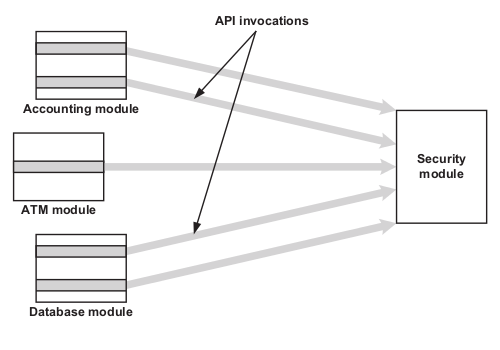
\includegraphics[scale=0.5]{images/Code_Scattering.png}
\caption{A representation of code scattering and code tangling.}
\label{fig:Code_Scattering}
\end{figure}\\
\\
AOP works by identifying join points, which are certain points during the execution of the program, e.g. a method call or execution. The set of all the join points is called the join point model. It is at these join points that we can modify the original program execution, which can go from something as simple as logging to something more invasive where the original code isn't even executed at all.\\
\\
To specify which join points we would like to interact with, a pointcut is used. Besides referring to a certain join point we also need a way to modify the execution of it. This is done by an advice, note that there can be multiple kinds of advice, e.g. before, after and around in AspectJ. In the end all these elements are put together by the weaver which results in woven code. The weaver will make sure that the advice is called at the join points identified by the pointcut it is connected to.\\
\\
The most well-known AOP language is AspectJ, which is an extension of Java. To demonstrate the concept of AOP a couple of AspectJ examples are shown here. In listing \ref{lst:AspectJ_Authenticator} a pointcut is specified that will match any deliver method of the MessageCommunicator, no matter the arguments or return type. Before this method is executed the user is authenticated.
\begin{lstlisting}[caption=An aspect to authenticate the user.,label=lst:AspectJ_Authenticator]
package ajia.security;
import ajia.messaging.MessageCommunicator;

public aspect SecurityAspect {
	private Authenticator authenticator = new Authenticator();

	pointcut secureAccess(): execution(* MessageCommunicator.deliver(..));
	
	before() : secureAccess() {
		System.out.println("Checking and authenticating user");
		authenticator.authenticate();
	}
}
\end{lstlisting}
Another example, shown in listing \ref{lst:AspectJ_Profiler}, determines the time required to execute any public method.
\begin{lstlisting}[caption=An aspect to profile methods.,label=lst:AspectJ_Profiler]
package ajia.profile;

public aspect ProfilingAspect {
	pointcut publicOperation() : execution(public * *.*(..));

	Object around() : publicOperation() {
		long start = System.nanoTime();
		Object ret = proceed();
		long end = System.nanoTime();
		System.out.println(thisJoinPointStaticPart.getSignature() + " took " + (end-start) + " nanoseconds");
		return ret;
	}
}
\end{lstlisting}

\section{Problem}
AOP is often implemented by extending an existing language, which often leads to a completely new language requiring new compilers and  breaking existing tools for the base language. Especially the latter is a reason why some people haven't made the step to start working with aspect-oriented languages.\\
\\
Though the concepts of AOP are quite general, which is reflected by the similarities in different aspect-oriented languages, all the AOP parts of these languages were written from scratch. The main reason for this is the absence of a general, language-independent library or framework to handle aspect-orientation. Another reason is that by building a language from scratch the developer gets more freedom to implement the desired features.

\section{Goal}
The goal of this thesis is to build such a framework that encloses all core ideas of AOP in an abstract manner without being specific about a particular base language. This should enable us to use the framework to develop an aspect-oriented language quicker and easier than currently is the case, by extending a couple of parts. The framework should be able to work for completely new base languages, and existing ones we want to extend. The latter one will pose the most problems as we wish to modify the existing compiler as little as possible. By making the framework abstract enough we want to ensure that it can be used for different types of base languages. 

\section{Overview}
The remainder of this thesis is structured as follows: in chapter \ref{chap:AOP_Components} the components of an aspect-oriented language are explained. In chapter \ref{chap:AOP_Framework} the developed framework is presented. In chapters \ref{chap:SmallC} and \ref{chap:Dot} the framework is instantiated for Small C and Dot. In chapters \ref{chap:AOWP}, \ref{chap:AspectMatlab} and \ref{chap:DiSL} we examine how some domain-specific aspect languages can be implemented using the framework. In chapter \ref{chap:Discussion} the current version of the framework is discussed, and the future work is presented in chapter \ref{chap:FutureWork}. Chapter \ref{chap:RelatedWork} discusses some related work and chapter \ref{chap:Conclusion} concludes the thesis.

\chapter{Aspect-Oriented Language Components}
\label{chap:AOP_Components}
An aspect-oriented language consists of several components. To explain these I will start from the base language and work my way up to get an aspect-oriented language. At every point I will make it more concrete with a small AspectJ example.\\
\\
The starting point of creating an aspect-oriented language is the base language, this is the existing language that we want to extend or is a completely new language. In the latter case the base language will be the new language excluding all the aspect-oriented features. The base language can be any kind of language: procedural, object-oriented, functional, logical, data-oriented, etc.\\
\\
After defining the base language we can define the join point model. This consists of all the points that occur during execution on which intervention of the aspects is allowed. The join point model itself is completely implicit, but it still is an important part of any aspect-oriented language as it is the link between the base language and the aspect-oriented part.\\
\\
Knowing at which points we can intervene doesn't allow us to do anything, we need a way to identify certain join points. This identification is done by using pointcuts, specifying one or more join points. Pointcuts make the join point model explicitly present in the aspect-oriented language. The way in which pointcuts allow us to refer to join points should be as close as possible to the way in which they appear in the base language. Listing \ref{lst:AspectJ_Pointcuts} shows two pointcuts. Both match the method 'bar' of an object 'Foo', though methodCall will match the call of it, and methodExec will match the execution.
\begin{lstlisting}[caption=Two method pointcuts.,label=lst:AspectJ_Pointcuts]
pointcut methodCall(): call(public void Foo.bar(int));
pointcut methodExec(): execution(public void Foo.bar(int));
\end{lstlisting}
 We use the example shown in listing \ref{lst:AspectJ_JoinPointShadow} to show the difference between the two pointcuts shown earlier. The pointcut 'methodCall' matches the actual call from 'callbar' while 'methodExec' matches the execution of the method itself.\\
\\
\begin{lstlisting}[caption=Example Java code.,label=lst:AspectJ_JoinPointShadow]
public class Foo {
	void bar(int i) {
		...
	}
}

public class CallFoo {
	void callbar() {
		bar(5);
	}
}
\end{lstlisting}
Now that we can refer to certain join points, we can actually start modifying the original code. This modification is encapsulated in an advice, which contains code that has to be executed. When this code should be executed is defined by the pointcut with which the advice is associated. An example of how this connection is established in AspectJ is shown in listing \ref{lst:AspectJ_Advice}.
\begin{lstlisting}[caption=An example of an advice.,label=lst:AspectJ_Advice]
pointcut methodCall(): call(public void Foo.bar(int));

before(): methodCall() {
	System.out.println("Calling bar");
}
\end{lstlisting}
Whenever the program passes a join point that matches with the associated pointcut, this advice must be executed. The code in the advice should be written in the base language to prevent the user from learning an entire new language. The examples in listing \ref{lst:AspectJ_Authenticator} and \ref{lst:AspectJ_Profiler} clearly show that most part of the advice body consists of plain Java code. The advice should also be able to have access to information about the join point. In AspectJ there are two ways to pass information. A first one is by using arguments as shown in listing \ref{lst:AspectJ_PointcutArgument}, another is by using the special \textbf{thisJoinPoint} keyword as shown in listing \ref{lst:AspectJ_ThisJoinPoint}.
\begin{lstlisting}[caption=Example of argument passing between pointcut and join point.,label=lst:AspectJ_PointcutArgument]
pointcut methodCall(int i) : call(public  void Foo.bar(int) && args(i);

before(int o) : methodCall(o) {
	System.out.println("Calling bar with " + o);
}
\end{lstlisting}
\begin{lstlisting}[caption=Example of using the thisJoinPoint keyword.,label=lst:AspectJ_ThisJoinPoint]
before() : methodCall() {
	System.out.println("Calling " + thisJoinPoint);
}
\end{lstlisting}
One problem that arises is: what is suppose to happen if we encounter a join point at which multiple advice are to be executed? This can be either caused by multiple pointcuts matching to the join point, or multiple advice being associated with the same pointcut. The latter case can be easily solved as we can combine the two advice into one bigger advice, as shown in listing \ref{lst:MergeAdviceBefore} and \ref{lst:MergeAdviceAfter}.\\
\begin{minipage}{0.48\textwidth}
\begin{lstlisting}[caption=Two colliding advice.,label=lst:MergeAdviceBefore]
before(): fooCall() {
	System.out.println("Advice 1.");
}

before(): fooCall() {
	System.out.println("Advice 2.");
}
\end{lstlisting}
\end{minipage}\hfill
\begin{minipage}{0.48\textwidth}
\begin{lstlisting}[caption=Two possible merged versions of the advice.,label=lst:MergeAdviceAfter]
before(): fooCall() {
	System.out.println("Advice 1.");
	System.out.println("Advice 2.");
}

before(): fooCall() {
	System.out.println("Advice 2.");
	System.out.println("Advice 1.");
}
\end{lstlisting}
\end{minipage}\\
The first is a bit more tricky since one pointcut can match join points different from the other, which means we can't just combine them. Imagine the two pointcuts shown in listing \ref{lst:AspectJ_ConflictPointcut}, it is clear that they would both match a method call to 'foobar', but while the first also matches a call to the method 'foo' the second will not. The other way around the second will match a call to the method 'bar', but the first will not.
\begin{lstlisting}[caption=Overlapping pointcuts.,label=lst:AspectJ_ConflictPointcut]
pointcut fooCall(): call(public void *.foo*());
pointcut barCall(): call(public void *.*bar());
\end{lstlisting}
The solution to this is of course to introduce an ordering mechanism. This ordering can be either placed on the pointcuts or on the advice, in the first case we still need to make sure that there is only one advice for each pointcut though. In AspectJ this is done by specifying the advice in the file in the desired order. An example of this is shown in listing \ref{lst:AspectJ_Precedence} and its output in listing \ref{lst:AspectJ_PrecedenceOutput}.\\
\begin{minipage}{0.48\textwidth}
\begin{lstlisting}[caption=Example of declaring precedence.,label=lst:AspectJ_Precedence]
before(): fooCall() {
	System.out.println("Advice 1.");
}

around(): fooCall() {
	System.out.println("Begin.");
	proceed();
	System.out.println("End.");
}

before(): fooCall() {
	System.out.println("Advice 2.");
}
\end{lstlisting}
\end{minipage}\hfill
\begin{minipage}{0.48\textwidth}
\begin{lstlisting}[caption=Output of the ordered advice.,label=lst:AspectJ_PrecedenceOutput]
Advice 1
Begin
Advice 2
End
\end{lstlisting}
\end{minipage}\\
One final component we need, is something that will actually make sure that the advice are executed when the join points are encountered. The weaver will make this happen, and can do this in multiple ways. The easiest is compile-time-weaving, which comes down to a pre-processing step. A more advanced form is run-time-weaving, yet other forms are available depending on the base language.\\
\\
With the components specified above it is perfectly possible to create an aspect-oriented language. However, some features are still missing, e.g. communication between different advice is impossible. Since aspect-orientation is often presented as an extension of object-oriented programming it makes sense to introduce some form of module or container to encapsulate pointcuts and advice. By doing this we immediately have the advantages offered by object-oriented languages among which are reusability, inheritance and encapsulation. Some examples of how reuse of an aspect is done in AspectJ is shown in listing \ref{lst:AspectJ_ReUse}.
\begin{lstlisting}[caption=Possibilities to reuse aspects.,label=lst:AspectJ_ReUse]
public aspect ProgramPoints {
	public pointcut main(): execution(public * *.*(..));
	public pointcut expensive(): execution(* *.Calculator || *.Renderer).*(..));
}

public abstract aspect Profiling {
	int count = 0;
	abstract pointcut toProfile();
	after(): toProfile() {
		count++;
	}
}

public aspect MyProfiling extends Profiling {
	pointcut toProfile():
	ProgramPoints.expensive();
}
\end{lstlisting}
An overview of all the components and how they are linked together is shown in figure \ref{fig:Aspect_Components}. The weaver is not considered to be part of the aspect language, just like a compiler is not considered a part of the language.
\begin{figure}[h!]
\centering
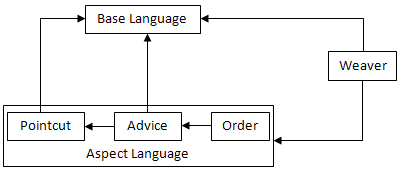
\includegraphics[scale=0.7]{images/AOF/Components.png}
\caption{An overview of the components.}
\label{fig:Aspect_Components}
\end{figure}

\chapter{Aspect-Oriented Framework}
\label{chap:AOP_Framework}
Since the framework has to be easily extensible to work with any kind of language it has to be very abstract and may not contain any information about a base language. On the other hand, creating a framework that is too abstract may require more effort from the developer in order to instantiate the framework with a particular base language, making the framework completely miss its goal. This means that the level of abstraction has to be well considered.\\
\\
First I will go into detail how the components that were identified in the previous chapter are represented and work in the framework. Then I will provide information about how the weaver works. Once all the components have been fully explained some remarks about the current version of the framework are made. To conclude the chapter I explain how we can now expand this framework to work with any base language.\\
\\
The first component of the aspect language that we identified are pointcuts. To completely specify a join point we need some way to identify its signature, this however is language specific and can therefore not be provided by the framework. Other common structures are arguments and context. The arguments are meant for information that can be used in the advice, while the context is a way to restrict matching join points based on  information that goes beyond the scope of the join point. The pointcut is implemented as an abstract Pointcut class.\\
\\
Letting an advice link to only one pointcut is too restrictive in some cases. It is easy to imagine we want an advice to be executed upon multiple join points. If these join points differ too much in signature it becomes impossible to describe them by one pointcut without also matching unwanted join points. This will result in duplicating the advice, to link it with more than one pointcut. It is for this reason that the framework provides a way to group those pointcuts in a set. Instead of linking advice to a single pointcut, they are now linked with an entire set. A set will match a join point if at least one of the pointcuts it contains matches the join point. Arguments can be made available for the advice by defining it in the set. All the pointcuts in that set will have to define those arguments on their own as well. A UML diagram of the PointcutSet and the Pointcut class can be seen in figure \ref{fig:PointcutSet}.\\
\begin{figure}[h!]
\centering
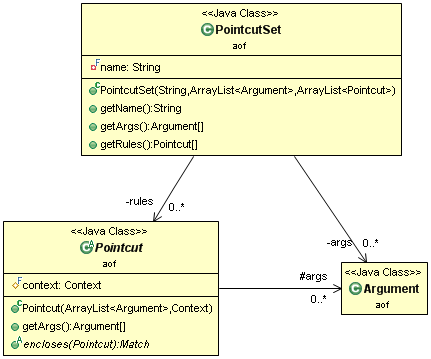
\includegraphics[scale=0.7]{images/AOF/PointcutSet.png}
\caption{UML diagram of the PointcutSet and Pointcut class.}
\label{fig:PointcutSet}
\end{figure}
\\
The advice are implemented by the abstract Advice class. This class has a name, which will make ordering them a lot easier, and a set of arguments. These arguments are the ones that can be used inside the advice body. Note that the arguments of the pointcutset to which this advice is linked to must be assignable to these arguments. The body or actual code of the advice is not provided by this class, simply because it depends on the base language as we want this to be in the same formalism. The UML diagram of the Advice class is shown in figure \ref{fig:Advice}.\\
\begin{figure}[h!]
\centering
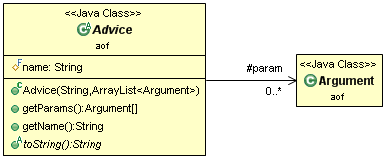
\includegraphics[scale=0.7]{images/AOF/Advice.png}
\caption{UML diagram of the Advice.}
\label{fig:Advice}
\end{figure}
\\
I already mentioned arguments and context but didn't explain how these are implemented. An argument is hard to abstract as every base language has its own vision of what an argument is. Though two concepts are very common, being a name and a type. For this reason the Argument class has a name, which is also required for access to the argument, and a type. While the name can be a string as this is general enough, the type is harder since it can not be a base language type, but should be more general. For this reason an interface called Type was created which allows the user to use his own type system. A UML diagram of this Argument class and the Type interface are shown in figure \ref{fig:Argument}.\\
\begin{figure}[h!]
\centering
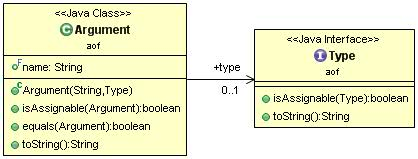
\includegraphics[scale=0.7]{images/AOF/Argument.jpg}
\caption{UML diagram of the Argument class.}
\label{fig:Argument}
\end{figure}
\\
A context is even more language dependent, which makes it impossible for the framework to provide more than the currently provided interface Context. Though there is a clear difference between arguments and context conceptually, this is however not often the case for real elements. Both context and arguments will often just contain a name and a value. In the current version of the framework the Context interface looks more like the Type interface, as can be seen by comparing the UML diagrams shown in figure \ref{fig:Type-Context} than the Argument class. I discuss this in more detail in chapter \ref{chap:FutureWork}.\\
\begin{figure}[h!]
\centering
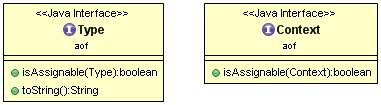
\includegraphics[scale=0.7]{images/AOF/Type-Context.jpg}
\caption{UML diagram of the Type and Context interface.}
\label{fig:Type-Context}
\end{figure}
\\
Different types of ordering exist: by assigning values, explicit linking, etc. The framework does not dictate the user which he has to use, instead he is free to choose whichever fits his needs. The user is also free to specify an order on either pointcuts or advice. Despite this freedom on the ordering 'language' the ordering itself is still limited. This is because the order has to be translated to a partial ordering of the advice.\\
\\
The weaver implemented as an abstract class, provides a way to register all components. The weaver is the part that connects everything together, since the advice does not keep a link to the pointcut itself, nor the other way around. This allows a better separation between pointcuts and advice and gives the weaver more freedom to operate.\\
\\
The actual weaving can not be done by the weaver as this depends on a lot of things such as preferences of the user and the base language. The framework does however provide some methods that simplify the weaving step. The most important one is 'executingAdvices', given a certain join point this method will return an ordered list of the advice that have to be executed. This ordering is done by the AdviceComparator, based on the partial ordering achieved from the ordering mechanism. This means that an advice in the list will be placed after all its predecessors. Note that the concept of predecessor has no meaning to the weaver. It is only used to return the ordered list. As an example we consider the partial ordering shown in figure \ref{fig:Order}. For this graph the weaver can return several ordered lists among which:
\begin{wrapfigure}{r}{0.65\textwidth}
\centering
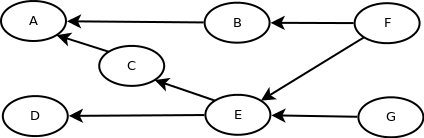
\includegraphics[scale=0.5]{images/AOF/Order.png}
\caption{A partial ordering of seven advice.}
\label{fig:Order}
\vspace{-80pt}
\end{wrapfigure}
\begin{itemize}
\item A; B; C; D; E; F; G
\item A; C; B; D; E; F; G
\item A; D; C; B; E; F; G
\item A; D; C; E; G; B; F
\item D; A; C; E; B; G; F
\end{itemize}
Which order is chosen is unpredictable, and it shouldn't matter as no order was specified among those elements.\\
\\
In case the user needs to know the pointcuts that match a certain joinpoint a method 'enclosingPointcuts' is provided. Both the 'executingAdvices' and 'enclosingPointcuts' return an instance of the Match class for each match they find. This 'match' is just an argument mapping from those specified in the join point to those that are specified in the advice or pointcut. This Match class, shown in figure \ref{fig:Match}, is used to get the join point specific value for an argument of the advice or pointcut.\\
\begin{figure}[h!]
\centering
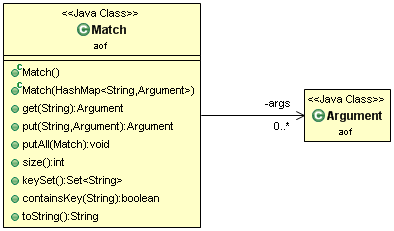
\includegraphics[scale=0.7]{images/AOF/Match.png}
\caption{UML diagram of the Match class.}
\label{fig:Match}
\end{figure}\\
The weaver also provides a way to specify input and output files. This is done by using the flags shown in \ref{tab:Flags}.\\
\begin{table}[h!]
\vspace{-10pt}
\centering
\begin{tabular}{l l}
-a \textit{files} & Specify the aspect files.\\ [0.5ex]
-s \textit{files} & Specify the source files.\\ [0.5ex]
-oDir \textit{dir} & Specify an output directory (optionally).\\
\end{tabular}
\caption{An overview of the flags available in the weaver.}
\label{tab:Flags}
\end{table}
\\
An UML diagram of the weaver, showing its complete API, is shown in figure \ref{fig:Weaver}.\\
\begin{figure}[h!]
\centering
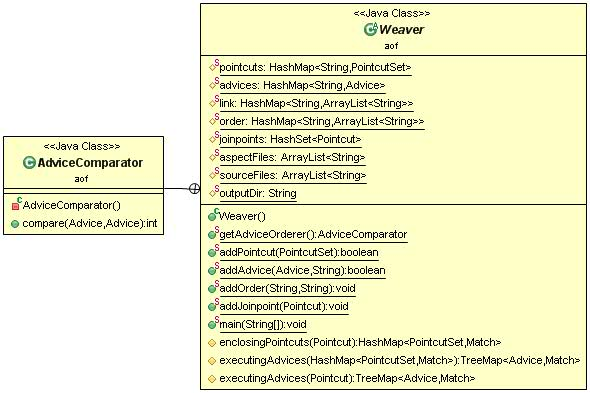
\includegraphics[scale=0.7]{images/AOF/Weaver.jpg}
\caption{UML diagram of the Weaver class.}
\label{fig:Weaver}
\end{figure}
\\
This concludes the explanation about all the components of the framework. A complete overview of the framework and how everything is connected can be seen in figure \ref{fig:FullView}.\\
\begin{figure}
\centering
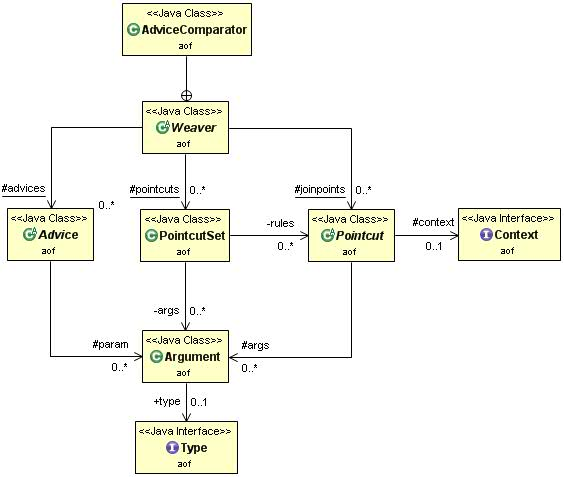
\includegraphics[scale=0.65]{images/AOF/Full.jpg}
\caption{UML diagram of the entire framework.}
\label{fig:FullView}
\end{figure}
\\
Some trade offs had to be made when designing the framework, which I will now discuss in more detail. First of all it needs to be noted that both Context and Type are interfaces which both specify only one method called 'isAssignable'. This means that Context and Type, though called different, do the same thing. We could use one general interface but this is not done to be able to handle future evolution.\\
\\
Adding a notion of aspect would allow a lot of nice features such as adding members, that can be used for communication between advice, and inheritance. Aspects could also be used as a way to encapsulate pointcuts and advice, though this can also be done without aspects simply by separating them over multiple files. Adding aspects to the framework would have introduced a lot of extra complexity. Since the goal of this thesis is to demonstrate the usability of such a framework, I have chosen to not include this but keep it as a future work.\\
\\
The framework uses an abstract notion of type, this is to achieve the level of abstraction required to separate the framework from the base language. This however means that for each base language we need a new type system that implements the Type interface, which might result in a lot of work. Sometimes it is however possible to use the same type system the compiler of the base language uses, if we can add the interface to it. Doing this would greatly reduce the cost of developing an AOP language.\\
\\
The advice and pointcuts are not directly connected with each other, the connection is achieved by the weaver. Because adding an explicit link does not provide any advantages, I have chosen to do it this way to ensure that the components are as loosely coupled as possible. Nevertheless the framework demands that at the moment a pointcut is added the pointcutset it is linked with must be be known to the compiler. This is a restriction in the current version of the compiler but can be easily solved by delaying this check until the actual weaving.\\
\\
Something that was not discussed so far is what happens if a join point is encountered that is matched by multiple pointcuts in the same pointcutset. In this case there basically are two options: either we execute the advice for each matched pointcut, or we only select the first matched pointcut of the set. Currently the latter is implemented in the framework, mostly because if we still want the first to happen, we can simply split the pointcutset.\\
\\
The base language compiler, or a modification of it has to extract join points from the source code. The join points that are generated will actually be instances of the Pointcut class. By doing this comparing whether a pointcutset contains a pointcut that matches the join point becomes trivial. Implementing both join points and poincuts as an instance of one class can be dangerous since they just aren't the same. One example is that poincuts can contain wildcards while join points can not. It may also be feasible to allow specifying types and sub-types in pointcuts to match multiple join points, where in the join point the types are fixed and known. This means that we have to use the Poincut class carefully if we use it for a join point.\\
\\
To conclude this chapter I will briefly explain how the framework can be instantiated to work with a base language. For more detailed examples I refer to chapters \ref{chap:SmallC} and \ref{chap:Dot} where the framework is instantiated for two different languages. Before being able to use the framework, the developer has to specify a language in which it is possible to specify pointcuts, advice and optionally an order. A parser has to be provided for this language, which will create the pointcuts and advice which are handed over to the weaver.\\
\\
The pointcuts and advice that have to be created have to be specific for the base language, this means that a subclass of Advice and one or more subclasses for Pointcut have to be created. The advice subclass is simple, it must contain the body of the advice. The pointcuts need to contain all information to identify a join point. Since there will be multiple types of pointcuts, one subclass has to be implemented for each type of pointcut. If desired a context can be added to the pointcut, by creating a class with the Context interface that contains all the context information to be used.\\
\\
The pointcuts and advice of course requires the developer to implement a type system. Depending on the availability of the type system used by the base language, and more precisely the compiler, it is possible to add small modifications to get the type system without much work. If not, this might be a bigger problem.\\
\\
Now we can create pointcuts and advice, we still need to expand the Weaver class to add the actual weaving. Since the framework gives us the advice to execute for each join point all the extended weaver has to do is generate code and weave the advice with the source code. This sounds easier than it sometimes is: It is especially important how we can interact with the base language. Eventually it all comes down to putting all the information in the weaver and generating the woven code. A schematic overview of this is shown in figure \ref{fig:Weaving}; note that the aspect language is split up into three components. It is possible to have this explicit separation, but most of the time this will cause more work to implement and thus not be this explicit.
\begin{figure}[h!]
\centering
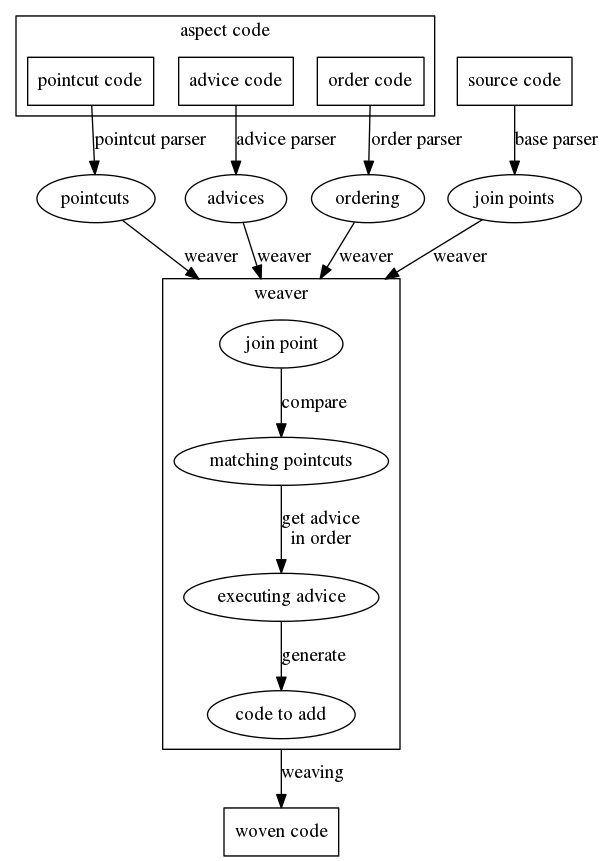
\includegraphics[scale=0.45]{images/AOF/Weaving.png}
\caption{Schematic overview of the weaving process.}
\label{fig:Weaving}
\end{figure}

\chapter{Small C}
\label{chap:SmallC}
To demonstrate the use of our framework in practice, it has been instantiated for a number of base languages. In this section the framework is applied to Small C.\\
\\
Small C is a subset of the procedural C language. Though it does not support structs or including other files, it does give us a good overview of what aspect orientation in a procedural programming language is like. As the source code of a compiler for this language was already available, this made Small C an interesting first step to test the framework.\\
\\
Despite the resemblance with C, I specify an example in listing \ref{lst:SmallC_Example}, to show the normal structure of a Small C program. This example will also be used later to demonstrate the functionality of the framework.
\begin{lstlisting}[language=C, multicols=2, caption=A simple Small C program., label=lst:SmallC_Example]
#include <stdio.h>

int count = 0;

int mySquare(int a) {
	return a * a;
}

int mySqrt(int a) {
	int i = 1;
	while (mySquare(i) <= a) {
		i = i + 1;
	}	
	return i - 1;
}

void main () {
	int a = 2;
	int b = 10;
	
	x = mySquare(a);
	count = count + 1;
	x = mySqrt(a);
	count = count + 1;
	x = mySqrt(25);
	count = count + 1;
	x = mySquare(count);
	count = count + 1;
}
\end{lstlisting}

\section{Join Point Model}
Due to the minimalistic character of the language the join point model is limited too. The join points identified can be divided into two groups, each with two types. An overview of the join points is given in table \ref{tab:SmallC_JoinPoints}.
\begin{table}[h!]
\centering
\begin{tabular}{|l|l|l|}
\hline
Join Point & Type & Description\\
\hline
\multirow{2}{*}{Function} & Call & The moment a function is called.\\
& Execution & The moment a function is executed\\
\hline
\multirow{2}{*}{Global Variable} & Set & The moment a global variable is set.\\
& Get & The moment a global variable is accessed.\\
\hline
\end{tabular}
\caption{Small C join points.}
\label{tab:SmallC_JoinPoints}
\end{table}

\section{Base Language Compiler}
Because the join points match some of the basic elements of the language, it was easy to find the interesting points in the compiler. At these points the compiler would already gather all the required information as it needed them itself to build the AST. This minimizes the code that was required to add leaving only some extra code to create the specific join point and to convert arguments to a type that could be used by the framework.

\section{Aspect Language}
Before discussing the parts of the framework it is required to explain some basic elements of the language. Though the language is mostly based on AspectJ, there are some differences mostly caused by the attempt to keep the language as simple as possible.\\
\\
In order to address multiple variables or functions simultaneously, the concept of wildcards is often introduced. This is also the case for this language, the '..' wildcard allows the user to specify a space that can be covered by any 0 or more characters.\\
\\
The compiler I used already had an entire type system, which could easily be modified to be used for the framework too. All that was required was making the CType class implement the Type interface. To support wildcards an extra type, the AnyType, was added. Note that it is impossible to partly specify a type such as '..int' which could match types such as longint, shortint and int. This is not a problem since the only types allowed in Small C are: 'int', 'float', 'char', 'void' and 'boolean' in combination with the array and pointer additions. An overview of the type system is shown in figure \ref{fig:CType}.\\
\begin{figure}[h!]
\centering
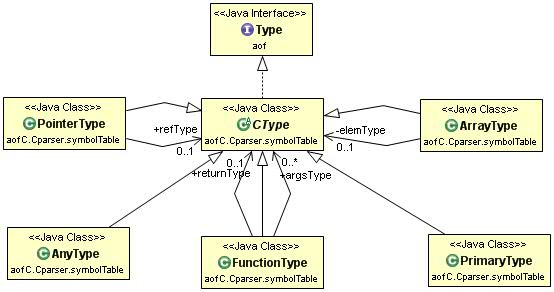
\includegraphics[scale=0.7]{images/AOFC/CType.jpg}
\caption{UML diagram of the CType class and its subclesses.}
\label{fig:CType}
\end{figure}
\\
A complete overview of the language in EBNF notation can be seen in listing \ref{lst:SmallC_EBNF}. Examples of the language will be given later, when each part is explained.\\
\begin{minipage}{\linewidth}
\begin{lstlisting}[caption=EBNF notation of the aspect langauge, label=lst:SmallC_EBNF]
file ::= (WS | order | pointcut | advice)* EOF
pointcut ::= 'pointcut' WS NAME WS? '(' args ')' WS? '{' rules '}'
rules ::= (WS | method | member)*
member ::= ('set' | 'get') WS type WS NAME WS? ';'
method ::= ('call' | 'execute') WS type WS NAME WS? '(' args ')' WS? ';'
advice ::= ('advice' WS NAME WS? ':' WS? )? ('before' | 'after' | 'around') WS NAME WS? '(' args ')' WS? '{' .* '}' 
order ::= 'order' WS? '{' WS? NAME (WS? ';' WS? NAME)* WS? '}' 
args ::= (type (WS NAME)? (WS? ',' WS? type (WS NAME)? )* )?
type ::= NAME ('[' ']' | '*')?

NAME ::= (LETTER | SPECIALCHARS | '..') (LETTER | DIGIT | SPECIALCHARS | '..')* 
WS ::= (' ' | '\n' | '\t' | '\r')+
OTHERCHARS ::= ~(LETTER | DIGIT | SPECIALCHARS)
DIGIT ::= '0..9'
LETTER ::= ('a..z' | 'A..Z')
SPECIALCHARS ::= ('*' | '_')
\end{lstlisting}
\end{minipage}

\section{Pointcuts}
All the kind of join points are mapped to pointcuts in a one-on-one manner. Which means that there two pointcuts classes, being MethodPointcut and MemberPointcut. The different types are handled by adding a flag to the pointcut. Because identifying a method or a global variable is completely different we need to separate these two. However, because a call and an execution both execute on a method we can combine these two together. This also holds for the get and set of a global variable.\\
\\
To identify a method join point we need the signature of the method, consisting of the name of the method, the return type and a set of arguments. The arguments are already implemented by the abstract super class, and thus are not part of the MethodPointcut class. A UML diagram for the MethodPointcut class is shown in figure \ref{fig:MethodPointcut}. Wildcards can be used in every element of the pointcut: in the name of the method, as a type of an argument, as  return type or as part of the argument list. Examples of the pointcuts are shown later when discussing each type in more detail. For now I show how wildcards can be used in listing \ref{lst:SmallC_Wildcards}.\\
\begin{figure}[h!]
\centering
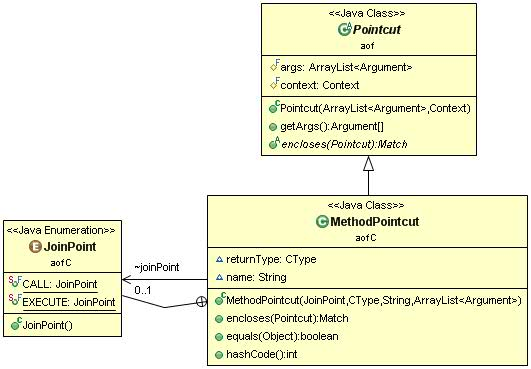
\includegraphics[scale=0.7]{images/AOFC/MethodPointcut.jpg}
\caption{UML diagram of the MethodPointcut class.}
\label{fig:MethodPointcut}
\end{figure}
\\
\begin{lstlisting}[multicols=2,caption=Some examples of pointcuts.,label=lst:SmallC_Wildcards]
pointcut p() {
	call int my..();
}

pointcut q() {
	call int mySquare(..);
}

pointcut r() {
	get int ..;
}

pointcut s() {
	get .. count;
}
\end{lstlisting}
It is not allowed to use a wildcard in the name of the arguments since these will be passed on to the advice to be used there, doing this wouldn't make any difference because the arguments are only matched on type and not on name. The names however are used to map them onto the arguments specified in the pointcutset. It is therefore also required that a pointcut contains all the arguments the enclosing pointcutset defines. An example of two method pointcuts are shown in listings \ref{lst:SmallC_MethodPointcutCall} and \ref{lst:SmallC_MethodPointcutExecute}, these pointcuts match respectively the calling and the execution of a method 'mySquare'.\\
\begin{minipage}{0.42\textwidth}
\begin{lstlisting}[language=C, caption=Example of a method call pointcut, label=lst:SmallC_MethodPointcutCall]
pointcut p() {
	call int mySquare(int);
}
\end{lstlisting}
\end{minipage}\hfill
\begin{minipage}{0.42\textwidth}
\begin{lstlisting}[language=C, caption=Example of a method execution pointcut, label=lst:SmallC_MethodPointcutExecute]
pointcut p() {
	execute int mySquare(int);
}
\end{lstlisting}
\end{minipage}
\\
The MemberPointcut is pretty empty, simply because the best way to identify a global variable is to see it as an argument of the pointcut. By doing this the only thing the MemberPointcut class has to add is the flag to identify the different types, as can be seen in the UML diagram shown in figure \ref{fig:MemberPointcut}. Just as with the MethodPointcut it is possible to use a wildcard as type, but it is also allowed to specify a wildcard as (part of) the name of the member to match multiple global variables. Because a MemberPointcut only contains one argument, being the member, it is always this argument that is mapped to the pointcutset argument. Since every pointcut needs to declare each pointcut defined by the pointcutset, a pointcutset that contains a member pointcut can only have one argument. An example of two member pointcuts are shown in listings \ref{lst:SmallC_MemberPointcutGet} and \ref{lst:SmallC_MemberPointcutSet}, these pointcuts match respectively the getting and setting of a global variable 'count'.\\
\begin{figure}[h!]
\centering
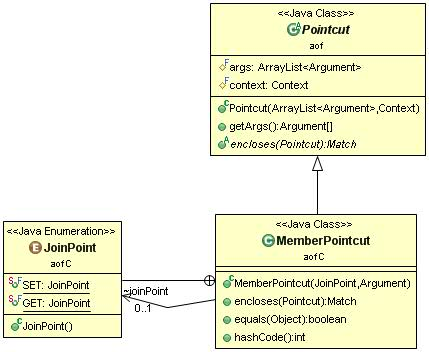
\includegraphics[scale=0.7]{images/AOFC/MemberPointcut.jpg}
\caption{UML diagram of the MemberPointcut class.}
\label{fig:MemberPointcut}
\end{figure}\\
\begin{minipage}{0.42\textwidth}
\begin{lstlisting}[language=C, caption=Example of a member get pointcut, label=lst:SmallC_MemberPointcutGet]
pointcut p() {
	get int count;
}
\end{lstlisting}
\end{minipage}\hfill
\begin{minipage}{0.42\textwidth}
\begin{lstlisting}[language=C, caption=Example of a member set pointcut, label=lst:SmallC_MemberPointcutSet]
pointcut p() {
	set int count;
}
\end{lstlisting}
\end{minipage}
\\
The current implementation does not use the context of the framework, which limits usability. However, I am convinced that adding a context would not add much functionality since the only context in Small C is the call hierarchy. Note that due to the lack of a context in the pointcuts the method call and execution pointcut will yield the same result, with a context we could for instance get the current method.

\section{Advice}
The advice is implemented as an CAdvice class shown in figure \ref{fig:CAdvice}. This class contains a string which represents Small C code. The code is allowed to contain arguments that are defined by the pointcutset it is linked to, but these are not treated specially in the CAdvice class itself. Besides the code, the CAdvice class also contains a flag to indicate the type. We distinguish three types of advice, specifying the moment of execution: before, after and around. These are the same as are present in AspectJ, and are straightforward. These types break the clear separation between pointcuts and advice and can be considered to be bad programming, yet this way we can create pointcutsets that are more reusable.\\
\begin{figure}[h!]
\centering
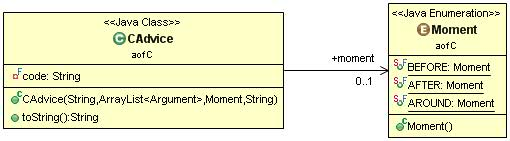
\includegraphics[scale=0.7]{images/AOFC/CAdvice.jpg}
\caption{UML diagram of the CAdvice class.}
\label{fig:CAdvice}
\end{figure}
\\
While the before and after can only be used to add extra code, the around advice can be used to skip the original code, or modify the values of the parameters. The \textbf{proceed()} call can be used to jump to the original join point (or the next advice, if any). Join points getting or setting a global variable are seen as a typical getter or setter and are treated the same as methods. Note that if the join point has a return type, either a method with a return type or a getter for a variable, the value will be returned by the \textbf{proceed()} call and it is the responsibility of the user to capture this.\\
\begin{minipage}{0.42\textwidth}
\begin{lstlisting}[caption=Example of a before advice, label=lst:SmallC_BeforeAdvice]
advice b: before p() {
	printf("Advice B\n");
}
\end{lstlisting}
\begin{lstlisting}[caption=Example of an after advice, label=lst:SmallC_AfterAdvice]
advice a: after p() {
	printf("Advice A\n");
}
\end{lstlisting}
\end{minipage}\hfill
\begin{minipage}{0.42\textwidth}
\begin{lstlisting}[caption=Example of an around advice, label=lst:SmallC_AroundAdvice]
advice c: around p() {
	printf("BEGIN C!\n");
	proceed();
	printf("END C!\n");
}
\end{lstlisting}
\end{minipage}
\\
An advice needs to be linked with a pointcutset, this is done by referring to it's name and specifying the arguments it requires. Note that the arguments need to match on type, but may differ on name. The names declared by the linked pointcutset can be used in the body of the advice.\\
\begin{minipage}{\linewidth}
\begin{lstlisting}[caption=Example of arguments.,label=lst:SmallC_Arguments]
pointcut p(int i) {
	call int mySquare(int i);
}

advice a: before p(int v) {
	printf("BEGIN: %i\n", v);
}
\end{lstlisting}
\end{minipage}\\
The body of the advice is not parsed in any way, at the moment it is created. It is not even parsed anywhere in the entire process until the very end which is simply compiling the woven code. This makes it possible to achieve communication between advice by using global variables of the original source code.

\section{Order}
There are two situations in which multiple advice can be mapped to the same moment in execution. The most obvious situation is when multiple advice are linked to the same pointcutset, but also if we have multiple pointcutsets that happen to match the same join point. In both cases it is possible that advice give rise to conflicts, but only if their types overlap.\\
\\
First, we will discuss the natural order of the advice. If there is no conflict the order is determined by the type of the advice, if there is a conflict but no order, it's up to the framework to resolve it. The location of the advice compared to the join point is shown in figure \ref{fig:COrder}. An overview of all the possible conflicts is more convienently shown in table \ref{tab:SmallC_Conflicts}.
\begin{figure}[h!]
\centering
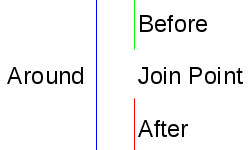
\includegraphics[scale=0.7]{images/AOFC/Order.png}
\caption{The location of the advice.}
\label{fig:COrder}
\end{figure}\\
\begin{table}[h!]
\centering
\begin{tabular}{l|c|c|c}
& before & after & around\\
\hline
before & + & - & + \\
\hline
after & - & + & + \\
\hline
around & + & + & +\\
\hline
\end{tabular}
\caption{An overview of the possible conflicts.}
\label{tab:SmallC_Conflicts}
\end{table}\\
To determine the order when conflicts do arise it is possible to specify an order between any two advice, even those that can never cause a conflict. This may seem useless, but it becomes useful in cases where we want more than two advice to be in a specific order and they are of different types. An order is specified as a list of advice, in which a later advice is closer to the join point than an earlier one. An example of specifying an order is shown in listing \ref{lst:SmallC_OrderExample} and listing \ref{lst:SmallC_OrderExampleResult}: in this example \textit{jp} is used to denote the join point. The order specified here compares a before and after advice but will have no effect as they can never cause a conflict. Note that it is possible to switch the before and after advice in the order and still get the same result.\\
\begin{minipage}{0.42\textwidth}
\begin{lstlisting}[caption=An example of a non-trivial order, label=lst:SmallC_OrderExample]
order{c; b; a}

advice b: before p() {
	printf("Advice B\n");
}

advice a: after p() {
	printf("Advice A\n");
}

advice c: around p() {
	printf("BEGIN C!\n");
	proceed();
	printf("END C!\n");
}
\end{lstlisting}
\end{minipage}\hfill
\begin{minipage}{0.42\textwidth}
\begin{lstlisting}[caption=The result of the order, label=lst:SmallC_OrderExampleResult]
printf("BEGIN C!\n");
printf("Advice B\n");
jp;
printf("Advice A\n");
printf("END C!\n");
\end{lstlisting}
\end{minipage}\\
The example shown in listing \ref{lst:SmallC_OrderExample2} and \ref{lst:SmallC_OrderExample2Result} shows an implicit order between a before and after advice where an after advice comes before a before advice.\\
\begin{minipage}{0.42\textwidth}
\begin{lstlisting}[caption=An example of a non-trivial order, label=lst:SmallC_OrderExample2]
order{a; c; b}

advice b: before p() {
	printf("Advice B\n");
}

advice a: after p() {
	printf("Advice A\n");
}

advice c: around p() {
	printf("BEGIN C!\n");
	proceed();
	printf("END C!\n");
}
\end{lstlisting}
\end{minipage}\hfill
\begin{minipage}{0.42\textwidth}
\begin{lstlisting}[caption=The result of the order, label=lst:SmallC_OrderExample2Result]
printf("BEGIN C!\n");
printf("Advice B\n");
jp;
printf("END C!\n");
printf("Advice A\n");
\end{lstlisting}
\end{minipage}

\section{Weaver}
The weaver is the largest piece of code. After all it is the core part of every aspect-oriented language. Once it has all the information it can start putting it together; it does this by writing wrapper methods for the join points, even if there is no advice to be execute for this join point. This will cause writing a lot of dummy wrappers, which do nothing more than just forwarding the call. These wrappers could have been omitted, but for simplicity they are not. Which wrappers are generated depends on the join point, and partly on the advice. For every global variable declared there will be two wrappers, one to handle the access to the variable, and another for the assignment of a new value. The same holds for a method but with call and execution instead. An example of these wrappers is shown in listing \ref{lst:SmallC_WrapperVariable} and \ref{lst:SmallC_WrapperMethod}. The original operations will be modified so that they use the wrappers instead. An example of these changes is shown in listing \ref{lst:SmallC_WrapperUsageBefore} and \ref{lst:SmallC_WrapperUsageAfter}.\\
\begin{minipage}{0.45\textwidth}
\begin{lstlisting}[language=C, caption=Example of variable wrappers, label=lst:SmallC_WrapperVariable]
int count_get_() {
	int _result_;
	_result_ = count;
	return _result_;
}

void count_set_(int _new_) {
	count = _new_;
}
\end{lstlisting}
\end{minipage}\hfill
\begin{minipage}{0.45\textwidth}
\begin{lstlisting}[language=C, caption=Example of method wrappers, label=lst:SmallC_WrapperMethod]
int mySqrt_exec_(int a) {
	int _result_;
	_result_ = mySqrt(a);
	return _result_;
}

int mySqrt_call_(int a) {
	int _result_;
	_result_ = mySqrt_exec_(a);
	return _result_;
}
\end{lstlisting}
\end{minipage}\\
\begin{minipage}{0.45\textwidth}
\begin{lstlisting}[language=C, caption=Example of code before weaving, label=lst:SmallC_WrapperUsageBefore]
x = mySqrt(25);
count = count + 1;
x = mySquare(count);
\end{lstlisting}
\end{minipage}\hfill
\begin{minipage}{0.45\textwidth}
\begin{lstlisting}[language=C, caption=Example of code after weaving, label=lst:SmallC_WrapperUsageAfter]
x = mySqrt_call_(25);
count_set_(count_get_() + 1);
x = mySquare_call_(count_get_());
\end{lstlisting}
\end{minipage}\\
Beside these wrappers some other methods are generated as well. One for each advice of the type before or after, and one for each matching join point of an around advice. The reason the around advice needs multiple instances is that it might have to proceed to the original method. While this is not the case for the before and after advice, it is still much easier to put them in a separate method. Especially considering that such an advice can alter the values of arguments, but that these changes may not be passed on to the actual method. By placing them in a method this behavior is ensure by the Small C language. Listen \ref{lst:SmallC_GeneratedMethods} shows the generated methods for the advice specified in listings \ref{lst:SmallC_BeforeAdvice}, \ref{lst:SmallC_AfterAdvice} and \ref{lst:SmallC_AroundAdvice}.\\
\begin{lstlisting}[language=C, caption=Generated methods, label=lst:SmallC_GeneratedMethods]
void _a() {
	printf("Advice A\n");
}

void _b() {
	printf("Advice B\n");
}

void _c_myMethod_() {
	printf("BEGIN C!\n");
	{
		 myMethod();
	}
	printf("END C!\n");
}
\end{lstlisting}
Beside generating wrappers, the weaver is also responsible for delivering the right arguments to the advice. This is another situation that shows the advantages of putting an advice in a separate method, as we can keep the names that are used in the advice code. If the around advice contains a proceed() call, the weaver has to replace this with a call to the original method or next around advice. The arguments specified in the proceed must be preserved and passed on. In order not to complicate the weaver any further it is required that the user manages the declaration of a value to store the return result and explicitly return this value if a return value is required. The declaration, assigning the return value of the proceed() and returning the value all must occur separately. This is because it is possible that the weaver will insert calls to other advice before and after the proceed() call. An example of this is shown in listing \ref{lst:SmallC_ComplexAround}, where the around advice is generated using the order as specified in listing \ref{lst:SmallC_OrderExample}.\\
\begin{lstlisting}[language=C, caption=A generated method for an around advice with advice nested within, label=lst:SmallC_ComplexAround]
int _c_mySquare_(int a) {
	int retVal = 0;
	printf("BEGIN C!\n");
	{
		_b();
		retVal = mySquare(a);
		_a();
	}
	printf("END C!\n");
	return retVal;
}
\end{lstlisting}
\begin{figure}
\centering
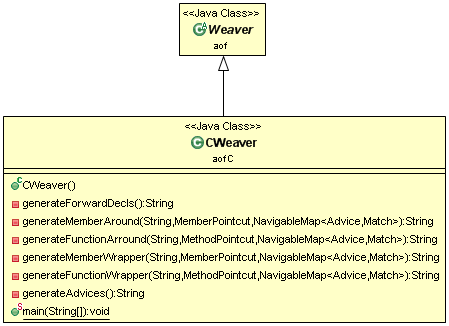
\includegraphics[scale=0.7]{images/AOFC/CWeaver.png}
\caption{UML diagram of the CWeaver class.}
\label{fig:CWeaver}
\end{figure}
Now that all the components have been introduced, I give a final overview of the entire structure in figure \ref{fig:CFull} to make it extra clear how all the components are connected.
\begin{figure}[h!]
\centering
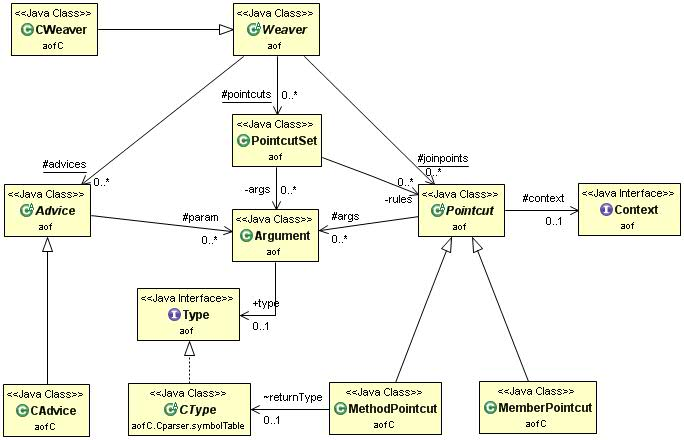
\includegraphics[scale=0.55]{images/AOFC/CFull.jpg}
\caption{A full overview of the use of the framework for Small C.}
\label{fig:CFull}
\end{figure}

\section{Example}
In this section a complete example is shown to get a better feeling of how all the pieces fit together.
\begin{lstlisting}[language=C, multicols=2, caption=Source code, label=lst:SmallC_ExampleSource]
#include <stdio.h>

int count = 0;

/* a^b */
int myPow(int a, int b) {
	int x;
	int result = 1;
	
	if (b <= 0) {
		return 1;
	}
	
	for (x = 1; x <= b; x = x + 1) {
		result = result * a;
	}
	
	return result;
}

/* a^2 */
int mySquare(int a) {
	return a * a;
}

/* square root of a. */
int mySqrt(int a) {
	int i = 1;
	while (mySquare(i) <= a) {
		i = i + 1;
	}
	
	return i - 1;
}

/* b-th root of a. */
int myRoot(int a, int b) {
	int i = 1;
	while (myPow(i, b) <= a) {
		i = i + 1;
	}
	
	return i - 1;
}

/* log_b(a) */
int myLog(int a, int b) {
	int i = 1;
	while (myPow(b, i) <= a) {
		i = i + 1;
	}
	
	return i - 1;
}

void main () {
	int a = 2;
	int b = 10;
	
	int x = myPow(a, b);
	count = count + 1;
	x = mySquare(a);
	count = count + 1;
	x = mySqrt(a);
	count = count + 1;
	x = mySqrt(25);
	count = count + 1;
	x = myRoot(1024, 2);
	count = count + 1;
	x = myLog(1024, 2);
	count = count + 1;
	x = mySquare(count);
}
\end{lstlisting}
\begin{lstlisting}[language=C, multicols=2, caption=The aspect code.]
order{b; c; a}

pointcut p(int x) {
	call int my..(int x, ..);
}

pointcut q(int i) {
	call int random(int i);
}

pointcut v(int count) {
	get int count;
}

advice getv: before v(int i) {
	printf("Count = %i\n", i);
}

advice a: after p(int i) {
	printf("BEGIN A\n");
}

advice b: after p(int i) {
	printf("BEGIN B\n");
}

advice c: around p(int i) {
	int retVal = 0;
	printf("BEGIN C!\n");
	retVal = proceed(i);
	printf("END C!\n");
	return retVal;
}
\end{lstlisting}
\begin{lstlisting}[language=C, multicols=2, caption=Woven code]
#include <stdio.h>

int count = 0;
int myPow(int a, int b) {
	int x = 0;
	int result = 1;
	if (b <= 0) {
		return 1;
	}
	
	for (x = 1; x <= b; x = x + 1) {
		result = result * a;
	}
	
	return result;
}

int mySquare(int a) {
	return a * a;
}

int mySqrt(int a) {
	int i = 1;
	while(mySquare_call_(i) <= a) {
		i = i + 1;
	}
	
	return i - 1;
}

int myRoot(int a, int b) {
	int i = 1;
	while(myPow_call_(i, b) <= a) {
		i = i + 1;
	}
	
	return i - 1;
}

int myLog(int a, int b) {
	int i = 1;
	while(myPow_call_(b, i) <= a) {
		i = i + 1;
	}
	
	return i - 1;
}

void main() {
	int a = 2;
	int b = 10;
	int x = myPow_call_(a, b);
	count_set_(count_get_() + 1);
	x = mySquare_call_(a);
	count_set_(count_get_() + 1);
	x = mySqrt_call_(a);
	count_set_(count_get_() + 1);
	x = mySqrt_call_(25);
	count_set_(count_get_() + 1);
	x = myRoot_call_(1024, 2);
	count_set_(count_get_() + 1);
	x = myLog_call_(1024, 2);
	count_set_(count_get_() + 1);
	x = mySquare_call_(count_get_());
}

void _getv(int i) {
	printf("Count = %i\n", i);
}

void _b(int i) {
	printf("BEGIN B\n");
}

void _a(int i) {
	printf("BEGIN A\n");
}

int count_get_() {
	int _result_;
	_getv(count);
	_result_ = count;
	return _result_;
}

int myPow_exec_(int a, int b) {
	int _result_;
	_result_ = myPow(a, b);
	return _result_;
}

void main_call_() {
	main_exec_();
}

int myLog_exec_(int a, int b) {
	int _result_;
	_result_ = myLog(a, b);
	return _result_;
}

int _c_myLog_(int i, int b) {
	int retVal = 0;
	printf("BEGIN C!\n");
	{
		retVal = myLog_exec_(i, b);
		_a(i);
	}

	printf("END C!\n");
	return retVal;
}

int myLog_call_(int a, int b) {
	int _result_;
	_result_ = _c_myLog_(a, b);
	_b(a);
	return _result_;
}

int mySqrt_exec_(int a) {
	int _result_;
	_result_ = mySqrt(a);
	return _result_;
}

int _c_myRoot_(int i, int b) {
	int retVal = 0;
	printf("BEGIN C!\n");
	{
		retVal = myRoot_exec_(i, b);
		_a(i);
	}

	printf("END C!\n");
	return retVal;
}

int myRoot_call_(int a, int b) {
	int _result_;
	_result_ = _c_myRoot_(a, b);
	_b(a);
	return _result_;
}

int mySquare_exec_(int a) {
	int _result_;
	_result_ = mySquare(a);
	return _result_;
}

int _c_mySqrt_(int i) {
	int retVal = 0;
	printf("BEGIN C!\n");
	{
		retVal = mySqrt_exec_(i);
		_a(i);
	}

	printf("END C!\n");
	return retVal;
}

int mySqrt_call_(int a) {
	int _result_;
	_result_ = _c_mySqrt_(a);
	_b(a);
	return _result_;
}

int _c_myPow_(int i, int b) {
	int retVal = 0;
	printf("BEGIN C!\n");
	{
		retVal = myPow_exec_(i, b);
		_a(i);
	}

	printf("END C!\n");
	return retVal;
}

int myPow_call_(int a, int b) {
	int _result_;
	_result_ = _c_myPow_(a, b);
	_b(a);
	return _result_;
}

void main_exec_() {
	main();
}

int myRoot_exec_(int a, int b) {
	int _result_;
	_result_ = myRoot(a, b);
	return _result_;
}

void count_set_(int _new_) {
	count = _new_;
}

int _c_mySquare_(int i) {
	int retVal = 0;
	printf("BEGIN C!\n");
	{
		retVal = mySquare_exec_(i);
		_a(i);
	}

	printf("END C!\n");
	return retVal;
}

int mySquare_call_(int a) {
	int _result_;
	_result_ = _c_mySquare_(a);
	_b(a);
	return _result_;
}
\end{lstlisting}

\section{Difficulties}
Despite having a modifiable compiler, there were a lot of problems of weaving the advice into the code. This was caused by the fact that the compiler was not designed to allow changes after parsing the code. Changing this would require big changes in the compiler and was therefore not really an option. Instead of changing the compiler another alternative was used, by creating two compilers, both with small changes, we could weave the file in multiple passes.\\
\\
The phases in which the woven code is generated are:
\begin{enumerate}
\item The source code will be parsed and all join points will be specified to the weaver. The weaver will produce wrappers and add these to a temporary output file.
\item The modified file will be parsed and the original calls will be modified to point to the wrappers.
\item The actual advice bodies will be written to the wrappers.
\item Compile the woven file with a regular compiler, this is not done by the weaver and has to be done by the user himself.
\end{enumerate}
It was impossible to change the calls in the first phase due to a simple circular dependency. The compiler checks that the called function actually exists. Since the compiler does not allow to add declarations before the current point, these declarations have to exist in the source code itself. To do this however we need to know which join points occur, and thus we need to have parsed the file before.\\
\\
Adding the content can not be done before phase 2, simply because the content contains function calls to the actual functions which need to be kept. Due to the way the compiler handles the code, it is impossible to distinguish a call from within a wrapper from one within a 'normal' function, yet we need to treat them separately. Therefore we need to add the content in a separate phase.

\chapter{Dot}
\label{chap:Dot}
In this section the framework is applied to Dot. Dot is a language that allows the user to easily specify the structure and appearance of a graph. Some of the features the language supports  are directed edges, undirected edges, subgraphs, labels for nodes and edges, different shapes, colors and more. Despite the fact that the language is quite easy-to-use, and has a straightforward syntax, it tends to be very verbose when trying to create large and complicated graphs.\\
\\
It is important to note that, unlike a typical aspect-oriented language, Dot does not have any notion of time or behavior as the result of the 'compiler' is the graph that the user wants. Because of this it adding AOP may seem somewhat strange since join points are defined as points during the execution of a program. Since the program does not execute, but only describes a static graph structure, all the join points simply map to points in the code in a static way. However, most ideas of AOP can still be applied.\\
\\
Because the syntax of Dot is that self-explanatory, the example showed in listing \ref{lst:Dot_Example} and the resulting graph in figure \ref{fig:Dot_Example} is enough to get an understanding of the language.\\
\begin{figure}
\begin{minipage}{0.45\textwidth}
\begin{lstlisting}[caption=The code to create a graph, label=lst:Dot_Example]
digraph G {
	subgraph cluster_0 {
		style=filled;
		color=lightgrey;
		node [style=filled,color=white];
		a0 -> a1 -> a2 -> a3;
		label = "process #1";
	}

	subgraph cluster_1 {
		node [style=filled];
		b0 -> b1 -> b2 -> b3;
		label = "process #2";
		color=blue
	}
	
	start -> a0;
	start -> b0;
	a1 -> b3;
	b2 -> a3;
	a3 -> a0;
	a3 -> end;
	b3 -> end;

	start [shape=Mdiamond];
	end [shape=Msquare];
}
\end{lstlisting}
\end{minipage}\hfill
\begin{minipage}{0.45\textwidth}
\centering
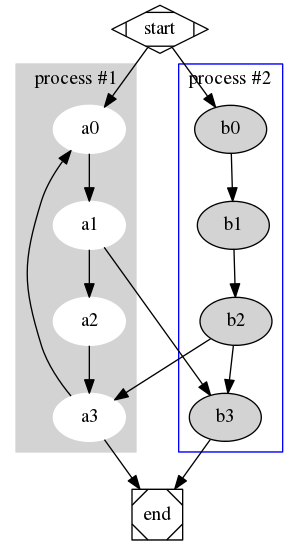
\includegraphics[width=\linewidth]{images/AOFDot/SmallExample.png}
\caption{The generated graph by dot.}
\label{fig:Dot_Example}
\end{minipage}
\end{figure}

\section{Join Point Model}
The join points identified in Dot are all the elements of the graph, being the graph itself, its nodes and edges. This simple join point model is mostly caused by the lack of run-time behavior.

\section{Base Language Compiler}
The compiler for the base language contains a parser that makes it possible to request all the graphs, nodes, and edges present in the file. Because of this no modifications were made to the base compiler.

\section{Aspect Language}
The aspect language mostly uses the same syntax as Dot itself to keep the language as simple as possible. There exists a wildcard to create more general rules, being '..'. By using this the programmer specifies that anything can take its place.\\
\\
Just as in Dot itself an graph, node and edge can contain attributes, these attributes are considered to be the arguments of the element and are used to restrict the matching. An attribute needs to have a name, being the attribute itself, and a value. For this value the wildcard can be used. It is also important to note that the wildcard can be used to denote any other attribute. Without this only elements with exactly those attributes are matched. Note that these attributes only act as arguments for the element and not for the pointcut.
\begin{lstlisting}[multicols=2,caption=Examples of using the wildcard.,label=lst:Dot_Wildcard]
node [label=..];
node [label="label", ..];
node [..];
.. [..];
\end{lstlisting}
It are the elements (node, edge, graph) that can be used as arguments, but to prevent having to make an entire type system for it, the id's of the elements are used instead. This makes it possible to keep the type system very basic, as can be seen in figure \ref{fig:DotType}.
\begin{figure}[h]
\centering
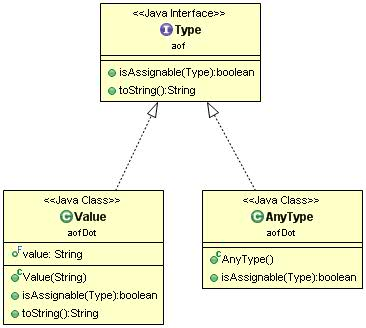
\includegraphics[scale=0.7]{images/AOFDot/DotType.jpg}
\caption{UML diagram of the type system for aspect orientation in Dot.}
\label{fig:DotType}
\end{figure}\\
There is no context information used, though it is possible to match elements based on the greater picture, being the graph they are part of. This will become clear when explaining the pointcuts and more specific the GraphPointcut.\\
\\
A complete overview of the language in EBNF notation is shown in listing \ref{lst:Dot_EBNF}.
\begin{lstlisting}[caption=EBNF notation of the aspect language., label=lst:Dot_EBNF]
file ::= (WS | order | pointcut | advice)* EOF
order ::= 'order' WS? '{' WS? NAME (WS? ';' WS? NAME)* WS? '}'
pointcut ::= 'pointcut' WS NAME WS? '(' args ')' WS? '{' rules '}' 
advice ::= ('advice' WS NAME WS? ':' WS? )? ('insert' | 'delete') WS NAME WS? '(' args ')' WS? '{' rules '}'
args ::= (WS? type WS NAME (WS? ',' WS? type WS NAME)* WS? )?

rules ::= (WS | graph | node ';' | edge ';')*
graph ::= ('..graph' | 'graph' | 'digraph' | 'subgraph') WS (NAME | '..') WS? '{' rules '}'
edge ::= (NAME WS? '=' WS? )? '(' WS? node WS? ')' WS? ('->' | '--') WS? '(' WS? node WS? ')' (WS? '[' attributes ']')?
node ::= (NAME | '..') (WS? '=' WS? (NAME | '..'))? (WS? '[' attributes ']')?
attributes ::= (NAME WS? '=' WS? (NAME | '..') (WS? ',' WS? attributes)? | '..')
type ::= ('Node' | 'Edge' | 'Graph')

NAME ::= '..'? ((LETTER | DIGIT | '_' | '"' .* '"') '..'? )* 
WS ::= (' ' | '\n' | '\t' | '\r')+
DIGIT ::= '0..9'
LETTER ::= ('a..z' | 'A..Z')
\end{lstlisting}

\section{Pointcuts}
There exist three kind of pointcuts being GraphPointcut, NodePointcut and EdgePointcut which represent respectively a graph, node and edge. All of these pointcuts can have Dot attributes, which will be stored as arguments and thus are part of the superclass Pointcut. Because each pointcut also has specific information I will now discuss these three pointcuts into more detail.\\
\\
A NodePointcut is the easiest as it only has a name and attributes, and since attributes are already handled by the superclass all we need to do is add a name. A node matches a NodePointcut if it has the same name and all the attributes match. Two examples of such a node poincut are shown in listing \ref{lst:Dot_NodePointcut} and \ref{lst:Dot_NodePointcut2}.\\
\begin{minipage}{0.45\textwidth}
\begin{lstlisting}[caption=A node pointcut matching any node start, label=lst:Dot_NodePointcut]
pointcut n() {
	start [..];
}
\end{lstlisting}
\end{minipage}\hfill
\begin{minipage}{0.45\textwidth}
\begin{lstlisting}[caption=A node pointcut matching any node with only a color, label=lst:Dot_NodePointcut2]
pointcut n() {
	.. [color=..];
}
\end{lstlisting}
\end{minipage}
\\
An EdgePointcut isn't that much harder, as the compiler relates every edge to a source and target node. These two nodes are again represented by a NodePointcut, as this was the easiest solution. On top of that we also need to know whether the edge is directed or not, which is a simple boolean. An edge matches an EdgePointcut if they are both directed and the sources and targets match or if they are both undirected, the source and target node may be switched. Two examples of an edge pointcut are shown in listing \ref{lst:Dot_EdgePointcut} and \ref{lst:Dot_EdgePointcut2}.\\
\begin{minipage}{0.45\textwidth}
\begin{lstlisting}[caption=An edge pointcut matching any edge from start to main, label=lst:Dot_EdgePointcut]
pointcut n() {
	(start [..]) -> (main [..]) [..];
}
\end{lstlisting}
\end{minipage}\hfill
\begin{minipage}{0.45\textwidth}
\begin{lstlisting}[caption=An edge pointcut matching any edge to main with a specified label., label=lst:Dot_EdgePointcut2]
pointcut n() {
	(.. [..]) -> (main [..]) [label=.., ..];
}
\end{lstlisting}
\end{minipage}
\\
The GraphPointcut requires all the information of its nodes and edges. Instead of introducing new types for nodes and edges, it is easier to reuse the pointcuts to represent this. A graph also has a name, though this information is not used in the current version. Checking whether a graph matches with a GraphPointcut is very simple, we just need to compare the nodes and edges it contains. A wildcard can be used to indicated that the graph may contain more nodes and edges. Two examples of a graph pointcut are shown in listing \ref{lst:Dot_GraphPointcut} and \ref{lst:Dot_GraphPointcut2}.\\
\begin{minipage}{0.45\textwidth}
\begin{lstlisting}[caption=A graph pointcut matching any graph G with an edge from start to main, label=lst:Dot_GraphPointcut]
pointcut n() {
	graph G {
		(start [..] ->  main [..]) [..];
		.. [..];
		(.. [..]) -> (.. [..]) [..];
	}
}
\end{lstlisting}
\end{minipage}
\begin{minipage}{0.45\textwidth}
\begin{lstlisting}[caption=A graph pointcut matching any graph G with only three nodes., label=lst:Dot_GraphPointcut2]
pointcut n() {
	graph G {
		start [..];
		main [..];
		exit [..];
		(.. [..]) -> (.. [..]) [..];
	}
}
\end{lstlisting}
\end{minipage}
\\
An overview of all the pointcuts and their interactions is shown in figure \ref{fig:DotPointcuts}.
\begin{figure}[h!]
\centering
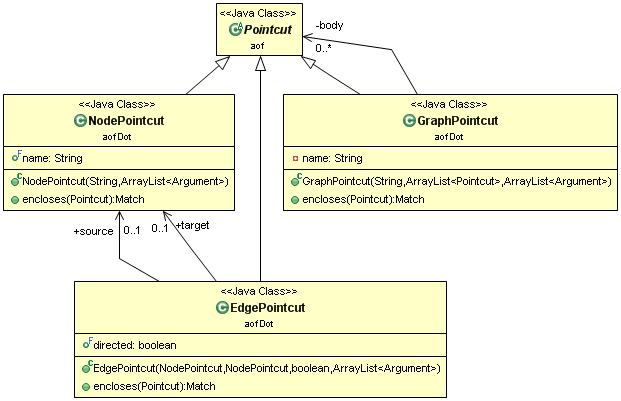
\includegraphics[scale=0.6]{images/AOFDot/DotPointcuts.png}
\caption{UML diagram of the three pointcut classes.}
\label{fig:DotPointcuts}
\end{figure}
\\
Arguments can be introduced on every level of the pointcut, which is shown by the examples in listing \ref{lst:Dot_Arguments}. Though the pointcut expresses the type of the argument, this is not really used by the weaver. As mentioned earlier it is the id of the elements that are used internally.
\begin{lstlisting}[caption=Examples showing the use of arguments, label=lst:Dot_Arguments]
pointcut n(Edge i, Node j) {
	graph .. {
		i = (main [..]) -> (j = .. [..]) [..];
		.. [..];
		(.. [..]) -> (.. [..]) [..];
	}
}

pointcut o(Node i) {
	i = .. [..];
}

pointcut p(Edge i) {
	i = (main [..]) -> (.. [..]) [..];
}
\end{lstlisting}
The current version does not use the context mechanism offered by the framework. It is however possible for the user to specify a form of context by using a graph pointcut. We can use an element inside this graph as an argument. Because the pointcut only matches that certain graph, we have specified some context information for the element we can use as argument.

\section{Advice}
There are two kinds of advice: insert and delete, which are meant to respectively insert elements or delete them from the graph. It is possible to add attributes to an element simply by creating an element that already exists but with the new attributes. Modifying an attribute is done in the same way. Deleting an attribute is done by specifying an attribute next to the element, if no such attribute is specified the entire element id deleted. By Using arguments it is possible to specify the elements that were matched in the pointcut. To provide this functionality the DotAdvice is created, which contains the type of the advice and the body, being the elements that have to be inserted or deleted. These elements are expressed using the Pointcuts; this allows us to quickly re-use all the functionality for the pointcuts, among which the usage of parameters and wildcards. An example of an advice is shown in listing \ref{lst:Dot_Advice}.
\begin{lstlisting}[caption=Some examples of advice., label=lst:Dot_Advice]
advice fn: insert n() {
	main [shape=box];
}

advice dn: delete n() {
	main [color=..];
}

advice in: insert n(Node i) {
	i [shape=box];
}

advice ie: insert n() {
	(main) -> (exit);
}
\end{lstlisting}
\begin{figure}
\centering
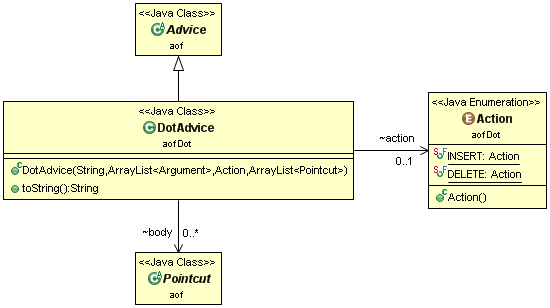
\includegraphics[scale=0.6]{images/AOFDot/DotAdvice.png}
\caption{UML diagram of the DotAdvice class.}
\label{fig:DotAdvice}
\end{figure}

\section{Order}
Despite the absence of runtime behaviour it is still possible that conflicts arise if two advice modify the same element and the modifications overlap. Consider an advice that colors a node red, and another that colors it blue. By changing the order of these two advice we either get a red node or a blue one. To specify an order, we simply create a semicolon separated list of the order in which they have to be executed. If there are two advice without an order that do execute at the same time, the order is undetermined. The following example demonstrates the difference in output caused by the order.\\
\begin{figure}[h!]
\centering
\begin{minipage}{0.45\textwidth}
\begin{lstlisting}[caption=The source code., label=lst:Dot_OrderOriginal]
digraph prof {
	start [color="blue"];
	main [color="green"];
	exit [color="red"];

	start -> main;
	main -> exit;
	start -> exit;
}
\end{lstlisting}
\end{minipage}
\begin{minipage}{0.45\textwidth}
\centering
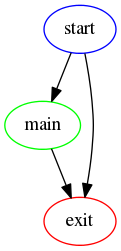
\includegraphics[scale=0.5]{images/AOFDot/Original.png}
\caption{Graph corresponding to \ref{lst:Dot_OrderOriginal}}
\end{minipage}
\end{figure}
\vspace{-20pt}
\\
\begin{lstlisting}[multicols=2,caption=An example of the order., label=lst:Dot_Order]
pointcut n(Node i) {
	i = start [..];
}

advice dn: delete n(Node i) {
	i [color=..];
}

advice fn: insert n(Node i) {
	i [color="red"];
}
\end{lstlisting}
\begin{figure}[h!]
\centering
\begin{minipage}{0.45\textwidth}
\centering
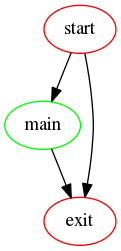
\includegraphics[scale=0.5]{images/AOFDot/Order1.png}
\caption{Result of executing dn before fn.}
\label{fig:Dot_Order}
\end{minipage}\hfill
\begin{minipage}{0.45\textwidth}
\centering
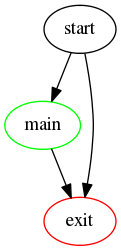
\includegraphics[scale=0.5]{images/AOFDot/Order2.png}
\caption{Result of executing fn before dn.}
\label{fig:Dot_Order2}
\end{minipage}
\end{figure}

\section{Weaver}
The weaver will first gather all information, i.e. join points, pointcuts and advice. After that it will start weaving the code. It is important to note that the weaver will first find all matching pointcuts for all join points before weaving. This is important as it means that if one advice modifies an element in such a way that it no longer matches a join point, any change caused by advice linked to that pointcut will still be executed.\\
\\
No other important notes are to be made. Thanks to the Dot compiler it is easy to get all the graphs, nodes and edges from a file modify them and write the resulting graph back to file. The UML diagram of the DotWeaver is shown in figure \ref{fig:DotWeaver}.\\
\begin{figure}[h!]
\centering
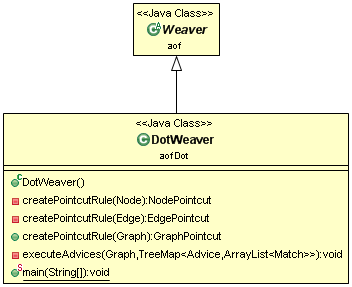
\includegraphics[scale=0.7]{images/AOFDot/DotWeaver.png}
\caption{UML diagram of the DotWeaver class.}
\label{fig:DotWeaver}
\end{figure}

\section{Example}
Now that all the basic elements are explained it is time to show a more complicated example. I will provide both the code and the visual graph before and after weaving.
\begin{lstlisting}[multicols=2, caption=The source code.]
digraph finite_state_machine {
	rankdir=LR;
	node [shape = circle];

	LR_0 [shape = doublecircle];
	LR_3 [shape = doublecircle];
	LR_4 [shape = doublecircle]
	LR_8 [shape = doublecircle];

	LR_0 -> LR_2 [label = "SS(B)"];
	LR_0 -> LR_1 [label = "SS(S)"];
	LR_1 -> LR_3 [label = "S($end)"];
	LR_2 -> LR_6 [label = "SS(b)"];
	LR_2 -> LR_5 [label = "SS(a)"];
	LR_2 -> LR_4 [label = "S(A)"];
	LR_5 -> LR_7 [label = "S(b)"];
	LR_5 -> LR_5 [label = "S(a)"];
	LR_6 -> LR_6 [label = "S(b)"];
	LR_6 -> LR_5 [label = "S(a)"];
	LR_7 -> LR_8 [label = "S(b)"];
	LR_7 -> LR_5 [label = "S(a)"];
	LR_8 -> LR_6 [label = "S(b)"];
	LR_8 -> LR_5 [label = "S(a)"];
}
\end{lstlisting}
\begin{figure}[h!]
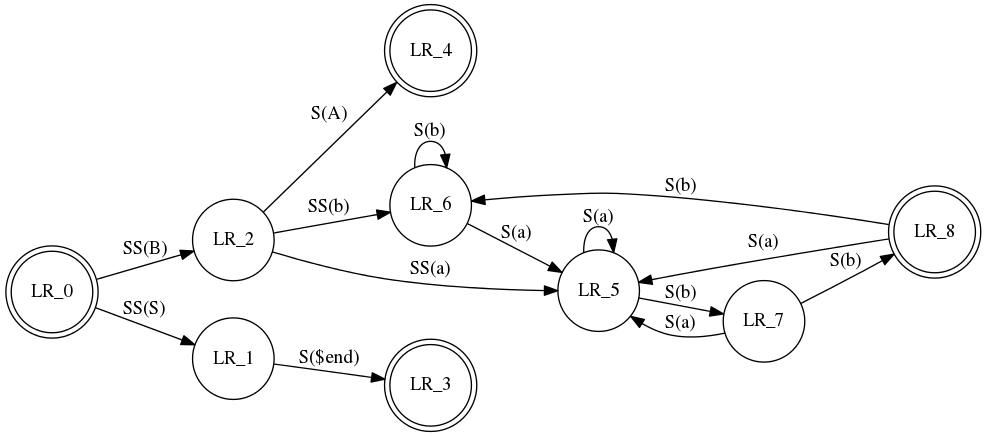
\includegraphics[width=\textwidth]{images/AOFDot/ExampleBefore.png}
\caption{The graph before weaving.}
\end{figure}
\begin{lstlisting}[multicols=2, caption=Aspect code.]
order{fn; color}

pointcut n(Node j) {
	j = LR_.. [..];
}

pointcut m(Edge j) {
	j = (.. [..]) -> (.. [shape=doublecircle, ..]) [..];
}

pointcut end(Node n) {
	n = .. [shape=doublecircle];
}

advice fn: insert n(Node j) {
	j [color=blue];
}

advice mark: insert m(Edge j) {
	j [color=red];
}

advice color: delete end(Node n) {
	n [color=..];
}

advice shape: insert end(Node n) {
	n [shape=box];
}
\end{lstlisting}
\begin{lstlisting}[multicols=2,caption=The woven code.]
digraph finite_state_machine {
	rankdir=LR;
	node [shape=circle];
	LR_0 [shape=box];
	LR_3 [shape=box];
	LR_4 [shape=box];
	LR_8 [shape=box];
	LR_2 [color=blue];
	LR_1 [color=blue];
	LR_6 [color=blue];
	LR_5 [color=blue];
	LR_7 [color=blue];
	
	LR_0 -> LR_2 [label=SS(B)];
	LR_0 -> LR_1 [label=SS(S)];
	LR_1 -> LR_3 [color=red, label=S($end)];
	LR_2 -> LR_6 [label=SS(b)];
	LR_2 -> LR_5 [label=SS(a)];
	LR_2 -> LR_4 [color=red, label=S(A)];
	LR_5 -> LR_7 [label=S(b)];
	LR_5 -> LR_5 [label=S(a)];
	LR_6 -> LR_6 [label=S(b)];
	LR_6 -> LR_5 [label=S(a)];
	LR_7 -> LR_8 [color=red, label=S(b)];
	LR_7 -> LR_5 [label=S(a)];
	LR_8 -> LR_6 [label=S(b)];
	LR_8 -> LR_5 [label=S(a)];
}
\end{lstlisting}
\begin{figure}[h!]
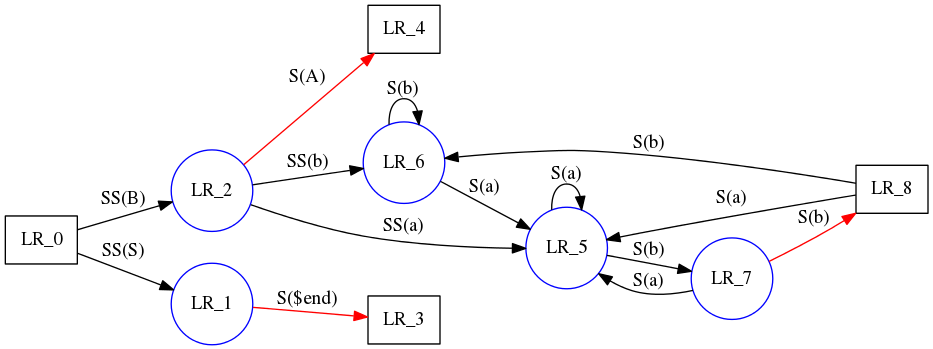
\includegraphics[width=\textwidth]{images/AOFDot/ExampleAfter.png}
\caption{The graph after weaving.}
\end{figure}

\section{Difficulties}
The biggest problem encountered was how to decide on the syntax of the aspect-oriented constructs in our extension of Dot. Once this was done adding aspect orientated programming went really fast, also thanks to the compiler which allowed it to easily modify the graph and write it back to file.\\
\\
One small problem was that there were two minor bugs in the compiler which needed to be fixed first, but this could be done really fast due to the availability of the source code.

\chapter{AOWP}
\label{chap:AOWP}
Due to the limited time available it is impossible to implement more languages using the framework. Instead I have chosen to examine existing languages and determine how they could be implemented with the framework.\\
\\
AOWP \cite{hokamura_aspect-oriented_2008} is a domain specific language for web applications. Most web applications are developed with the Model-View-Controller framework which clearly separates the application into business logic (model layer) and the visual component (view layer), which communicate through the controller.\\
\\
Although there exists an AOP language for PHP called AOPHP, this language has some flaws. First of all there is a lack of pointcuts to really cover all join points of web applications. Secondly there is no way to handle a history of page visits without modifying the web pages. Finally we note that the aspects can not be sufficiently separated from the crosscutting concerns.

\section{Join Point Model}
The join points that can occur in a web application consists of events based on HTTP and language specifications of well-known Web programming languages such as PHP and Java/Servlet. Where the first consists of receiving HTTP requests, reading form data and reading or writing cookie data, the latter consists of reading the session data. An overview of all the events is shown in table \ref{tab:AOWP_Events}.
\begin{table}
\centering
\begin{tabular}{l|l}
\hline
Abbreviation & Event\\
\hline
\hline
REQ & Receive an HTTP Request\\
\hline
F/R & Read the form data\\
\hline
C/R & Read the cookie data\\
\hline
C/W & Write the cookie data\\
\hline
S/R & Read the session data\\
\hline
S/W & Write the session data\\
\hline
\end{tabular}
\caption{AOWP events}
\label{tab:AOWP_Events}
\end{table}

\section{Aspect Language}
AOWP reuses the syntax of web programming languages such as PHP and Java/Servlet. It does this by mapping the aspect constructs onto object-oriented structures. By doing this the effort required by the user is minimized as he does not need to learn a new language.\\
\\
Creating an aspect can be done by creating a class that extends the Aspect class, adding a pointcut and an advice is done by declaring functions with the name of respectively 'pointcut' and the name of the type of advice ('before', 'after', 'around'). An example is shown in listing \ref{lst:AOWP_ExampleNews} and \ref{lst:AOWP_ExampleLoad}.\\
\\
This could also be accomplished if we were to use our framework, since it is required to create an aspect language of our own. This means that the same syntax could be chosen, though it has to be said that the framework has no notion of aspects, but this is not a problem as it is the responsibility of the compiler to extract the required information and provide it to the weaver in a format it understands.

\section{Pointcuts}
There are three categories of pointcuts, a first one selects events, a second selects event flows and a third selects based on usage contexts. Each of these categories has a set of sub-types, or so-called designators. An overview of all the designators are given in tables \ref{tab:Designators_AOWP_Events}, \ref{tab:Designators_AOWP_Flows} and \ref{tab:Designators_AOWP_Contexts}. How these designators are used can be seen in table \ref{tab:Designators_AOWP_Pointcut}. From this table we also see that it is possible to use regular expressions as an argument of a designator.\\
\begin{table}[h!]
\centering
\begin{tabular}{l|p{7cm}}
\hline
Designator & Description\\
\hline
\hline
request & Select REQ with the specified URL\\
\hline
getget & Select specified F/R in a GET request\\
\hline
postget & Select specified F/R in a POST request\\
\hline
cookieget & Select specified C/R\\
\hline
cookieset & Select specified C/W\\
\hline
sessionget & Select specified S/R\\
\hline
sessionset & Select specified S/W\\
\hline
\end{tabular}
\caption{Designators for selecting AOWP events}
\label{tab:Designators_AOWP_Events}
\end{table}
\begin{table}[h!]
\centering
\begin{tabular}{l|p{7cm}}
\hline
Designator & Description\\
\hline
\hline
withinrequest & Select all AOWP events in a REQ\\
\hline
pflow & Select all AOWP events in specified page transitions\\
\hline
\end{tabular}
\caption{Designators for selecting AOWP event flows}
\label{tab:Designators_AOWP_Flows}
\end{table}
\begin{table}[h!]
\centering
\begin{tabular}{l|p{7cm}}
\hline
Designator & Description\\
\hline
\hline
accessnum & Select all AOWP events when the number of access users is the specified number or greater.\\
\hline
\end{tabular}
\caption{Designators based on usage contexts}
\label{tab:Designators_AOWP_Contexts}
\end{table}
\begin{table}[h!]
\centering
\begin{tabular}{l|p{7cm}}
\hline
Example & Description\\
\hline
\hline
request(/news.php) & Selects all events of receiving HTTP requests on news.php.\\
\hline
withinrequest(/login.php) & Selects all events generedted during the execution of HTTP requests for login.php\\
\hline
pflow(/news.php) & Selects all the events involved in handling HTTP requests when the user has seen news.php\\
\hline
accessnum(5) & Selects all events involved in handling HTTP Requests when the number of users if 5 or more.\\
\hline
request(/*Action.php) & Selects the REQ whose name starts with '/' and ends with 'Action.php'.\\
\hline
!pflow(/news.php) & Selects a negative set of events selected by pflow(/news.php)\\
\hline
\end{tabular}
\caption{Examples of designator.}
\label{tab:Designators_AOWP_Pointcut}
\end{table}
\\
I will now discuss how these pointcuts could be implemented with the earlier presented framework. Instead of creating a pointcut subclass for each category it is more interesting to only create one subclasses being AOWPPointcut. I choose to take all the pointcuts together as there is no distinction in how these are represented. The AOWP designators shown in table \ref{tab:Designators_AOWP_Flows} will not become part of the pointcut, but instead will be added to the context. The class will rely on the arguments of the Pointcut superclass to implement the argument. The specific designator this instance represents has to be indicated by a special value, either an enum or an integer. \\
\\
By doing this we can easily specify pointcuts, creating join points is however a bit more tricky due to capturing the event flow. We could do this naively and create a pointcut for each element we encountered along the flow, but that would cause a long creation and comparison delay. It is much better to capture the entire flow as a context and provide that along with the join point. This means that checking whether a pointcut matches a join point is a bit more work, but it allows us to generate only one instance for the entire join point.\\
\\
AOWP allows combining multiple designators by using the negation (!), intersection (\&) and union ($|$) operator. This is not possible with the framework, since this only supports union. It is however not a big problems as we can create a new type of pointcut, the OperatorPointcut. This pointcut will simply execute a certain operator (!, \& or $|$) on its members, which are again pointcuts. Another approach could have been to use the union of the framework and using the OperatorPointcut only for the negation and intersection, but this would lead to some extra work to be done. We would have to rework some expressions to make the unions the top-level operator or remote them completely. This can be seen in the following examples. In these examples I use simple letters to represent pointcuts.
\begin{align*}
!\left(a | b\right) \& c & \Rightarrow \left(!a \& !b\right) \& c\\
\left(a | b \right) \& !c & \Rightarrow \left(a \& !c\right) | \left(b \& !c \right)
\end{align*}
To avoid this extra work it makes more sense to treat the union the same way as the negation and the intersection.

\section{Advice}
The types of advice AOWP supports is the same as AspectJ, being 'before', 'after' and 'around'. The body of an advice is normal code with extension of the \textbf{proceed()} call. In contrast to AspectJ, there are no variables for the context, all this information is provided as arguments of the advice..

\section{Weaver}
Due to the dynamic behaviour of web applications it is impossible to rely on compile time weaving, and thus run-time weaving is required. The weaver itself works pretty straightforward by extracting join point shadows and injects code to call the weaver.\\
\\
This would cause some problems when using the framework, as the current version does not support run-time weaving. A work-around is to set up the weaver each time it is required, but this introduces a large overhead for creating and loading the pointcuts each time. This is discussed in more detail in chapter \ref{chap:FutureWork}.

\section{Examples}
\begin{lstlisting}[caption=An advice to alert the user to check the newspage.,label=lst:AOWP_ExampleNews]
class NewsAlertAspect extends Aspect {
	/* !pflow(/news.php) & request(*) */	
	funcion Pointcut() {
		$pc = new Pointcut();
		$pc->addNotAnd(new PFlowPC("/news.php"));
		$pc->addAnd(new RequestPC("*"));
		return $pc;
	}
	
	function before($adviceContext) {
		alertToViewNews();
	}
}
\end{lstlisting}
\begin{lstlisting}[caption=An advice that alerts on heavy load.,label=lst:AOWP_ExampleLoad]
class LoadAlertAspect extends Aspect {
	/* accessnum(20) & request(*) */	
	funcion Pointcut() {
		$pc = new Pointcut();
		$pc->addAnd(new AccessNumPC(20));
		$pc->addAnd(new RequestPC("*"));
		return $pc;
	}
	
	function before($adviceContext) {
		alertForAccessTooMany();
	}
}
\end{lstlisting}
\section{Difficulties}
The language itself will not give rise to many problems if we would try to implement it with the framework. Only the requirement for run-time weaving is currently a problem, though there are some work-arounds these are not feasible and would require more work than if the framework would make it possible. I discuss this later again in chapter \ref{chap:Discussion}.

\chapter{AspectMatlab}
\label{chap:AspectMatlab}
In this chapter I examine how we could implement AspectMatlab by using the framework. AspectMatlab \cite{aslam_aspectmatlab:_2010}, as the name suggests, is an AOP extension to Matlab. Like other extensions it adds pointcuts and advice for method calls or execution and get or setting of variables. It does however more than just this, because Matlab has a strong focus on loops, it also adds pointcuts for loops.\\
\\
As presented in the paper on AspectMatlab it performs source to source compilation taking AspectMatlab source files as input and generating Matlab source files as output. The compiler was built using a couple of toolkits such as Natlab and MetaLexer to get a modular and extensible compiler.

\section{Join Point Model}
Besides the method calls and execution that are present in most languages, call and execution can also be applied for scripts which are commonly used in Matlab. Other commonly found join point such as get and set for arguments are also present. Aside from these, AspectMatlab also identifies three join point concerning loops, being the execution of the entire loop, the execution of the loop head and the execution of the loop body. This is because the loop is one of the main entities in an typical Matlab program.

\section{Base Language Compiler}
The base language compiler used in the paper is McLab, which is an extensible Matlab compiler. This comes in handy as we will want to modify it to report information and join points to the weaver.

\section{Aspect Language}
The main element of the language is an aspect. Such an aspect can contain properties and methods like a class, but more important it has patterns (pointcuts) and actions (advice). Each of these elements has a syntax similar to normal Matlab syntax as can be seen in listing \ref{lst:Matlab_ExampleCalls}.\\
\\
The main problem that arises if we want to implement this with the framework, is that there is no notion of 'aspect', which makes it impossible to have properties or methods related to it. If we would want to implement something similar as in the mentioned example, we would have to implement a class or script containing the methods and attributes to which we could write the code for the actions during weaving. This is however not very clean code, and we would be undermining the main goal of AOP, which is to clearly concentrate the concerns.\\
\\
Other cases however where we do not rely on attributes can be done without a problem. Also the presence of methods in the aspect files is not a problem as we can simply copy them to a new script or even directly into the advice that needs it.\\
\\
AspectMatlab provides the user with some context information in the form of context selectors. Which are present depends on which join point is encountered. Doing this with the framework can be done by specifying them as arguments. This is easier than using the context information as the Argument already has a name and a certain type. An overview of all the context selectors for different join point types are shown in table \ref{tab:Matlab_Context}.
\begin{table}[h!]
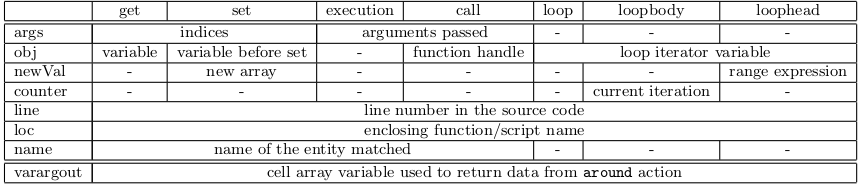
\includegraphics[width=\textwidth]{images/Languages/Matlab_Context.png}
\caption{Context selectors for different join point types.\citep{aslam_aspectmatlab:_2010}}
\label{tab:Matlab_Context}
\end{table}

\section{Pointcuts}
The pointcuts match the join points which were discussed earlier. therefore I will not discuss them any further but just show an overview in table \ref{tab:Matlab_Patterns}.\\
\begin{table}[h!]
\centering
\begin{tabular}{l|l}
\hline
Pointcut & Description\\
\hline
\hline
call & Captures all calls to functions/scripts.\\
execution & Captures the execution of function bodies.\\
get & Captures array accesses.\\
set & Captures array sets.\\
loop & Captures execution of all loops.\\
loophead & Captures the header of the loop.\\
loopbody & Captures the body of the loop.\\
\hline
\end{tabular}
\caption{List of patterns.}
\label{tab:Matlab_Patterns}
\end{table}\\
It is possible to further restrict the scope of matching by using the within pattern. On the other hand it is also possible to generalize pointcuts by using wildcards. The '*' wildcard can be used to match any function/variable or exactly one argument. The '..' wildcard can be used to match one or more variables.\\
\\
Because of the Matlab syntax, where 'foo(1,2)' could either be a call to a function with arguments '1' and '2' or an array indexation, it is possible to create a general notation for calling a function or script and getting or setting a variable. A list of possible matches is given in table \ref{tab:Matlab_PatternExamples}.\\
\begin{table}[h!]
\centering
\begin{tabular}{l|l}
\hline
Pointcut & Description\\
\hline
\hline
call(foo) & Matches all calls to foo.\\
call(foo()) & Matches calls to foo with no arguments.\\
call(foo(*)) & Matches calls to foo with exactly one argument.\\
call(foo(..)) & Matches calls to foo with 1 or more arguments.\\
call(foo(*,..)) & Matches calls to foo with 2 or more arguments.\\
call(*(*,..)) & Matches any call with two ore more arguments.\\
\hline
\end{tabular}
\caption{Selective pattern matching.}
\label{tab:Matlab_PatternExamples}
\end{table}\\
If we were to implement these pointcuts with the new framework we might end up with three subclasses for Pointcut. It is however possible to group them all together into one since there is no clear distinction between a function call and getting a variable. The within pattern would become part of the context provided to the pointcut.

\section{Advice}
AspectMatlab identifies three types of advice being before, around and after. The body of an advice is normal AspectMatlab code (possibly extended with the proceed() call) as can be seen in listing \ref{lst:Matlab_ExampleCalls}.\\
\\
As mentioned before, is it possible to provide context information to the advice. It is also possible to use variables specified within the aspect to communicate between advice or between multiple executions of the same advice. This latter one will cause the most problems as it is currently impossible to do anything like this with the framework. To solve this a work-around could be used where we use static data in the original matlab code can be used. This is however bad coding and breaks the entire concept of aspect-oriented programming.

\section{Order}
AspectMatlab introduces a default ordering where the first encountered around advice becomes the outermost one, followed by the rest of the around advice in the order of appearance. After the around advice, all before advice are placed in order of occurrence before the actual join point. The same holds for the after advice that are placed right after the join point in the order encountered before the around advice. This relation between before, after and around advice is shown visually in figure \ref{fig:AspectMatlab_Order}.\\
\begin{figure}[h!]
\center
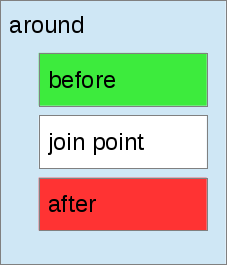
\includegraphics[scale=0.5]{images/Languages/AspectMatlab_Order.png}
\caption{A visual representation of the order between before, after and around advice.}
\label{fig:AspectMatlab_Order}
\end{figure}
\\
Since the framework does not provide such a default order, it is required for the AspectMatlab compiler to explicity add such an order to the weaver. This isn't very complicated though, it suffices to remember the last encountered advice of each type (before, around and after) so that when we read a new one we can add create a link between these two advice and mark the stored one as a predecessor of the new one.\\
\\
This solves the ordering problem between advice of the same type, what still remains is the order between the different types. There are two different approaches to solve this:
\begin{enumerate}
\item Create a link between the types.
\item Handle the different types one by one in the weaver.
\end{enumerate}
The first approach may sound like the best one, but at the same time it does some redundant work, simply because when weaving we will have to treat every type of advice differently. The different treatment is a direct result of the inherent difference between before, after and around advice. This means we could organize them during weaving according to their type.\\
\\
If however it is still preferred to have an order between the different types, which is possible as it might be helpful with certain implementations, this isn't much work to be done. To execute all before advice after the last around advice, we need to store the first encountered before advice. We need it at the end to define the last around advice as a predecessor of this first before advice. To make the last after advice happen before the last around advice, since this will be the deepest one and thus the first to be executed after the after advice, we need to define the last after advice as a predecessor of the last around advice. \\
\\
Because of the order behaviour caused by the around advice, which makes the order 'reflecting' over the join point. This leads to some confusing ordering and thus it can still not be used that straightforward.

\section{Weaver}
The AspectMatlab compiler (weaver) has been built using extensible toolkits, and aimed for a very clean and modular implementation. It takes a collection of Matlab and AspectMatlab source files as its input and produces a collection of woven Matlab source files. I will not discuss the entire process of how this is done, but a simple overview can be seen in figure \ref{fig:Matlab_Weaver}.\\
\begin{figure}[h!]
\centering
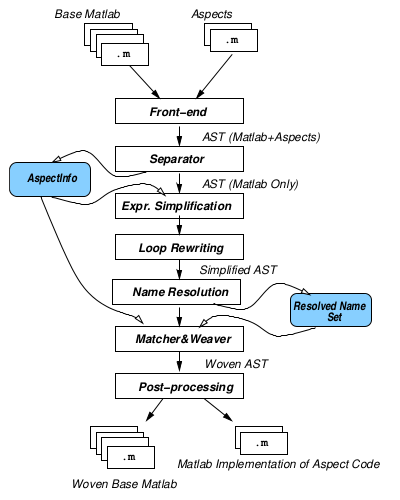
\includegraphics[scale=0.5]{images/Languages/Matlab_Weaver.png}
\caption{Overal structure of the amc AspectMatlab compiler. \citep{aslam_aspectmatlab:_2010}}
\label{fig:Matlab_Weaver}
\end{figure}
\\
To be able to call all the advice at the right point, some transformations are required. All compound expression are disassembled into simple expressions as can be seen in the following example:\\
\begin{minipage}{0.45\textwidth}
\begin{lstlisting}[caption=Original code.]
z = sum(x) / length(y);
\end{lstlisting}
\end{minipage}\hfill
\begin{minipage}{0.45\textwidth}
\begin{lstlisting}[caption=Resulting code.]
AM_CVar_5 = x;
AM_CVar_6 = sum(AM_CVar_5);
AM_CVar_7 = y;
AM_CVar_8 = length(AM_CVar_7);
z = (AM_CVar_6 / AM_C_Var_8);
\end{lstlisting}
\end{minipage}
\\
It is also important to note that, due to Matlab's semantics it is hard to determine at compile time the semantics of an expression. Because they wanted to minimize the amount of run-time checks, they introduced a name resolution analysis which adds extra information to the AST so they can determine the type.\\
\\
We could implement this the same way using the framework, without requiring any changes to the process.

\section{Examples}
\begin{lstlisting}[caption=An aspect to count all calls made with at least 2 arguments., label=lst:Matlab_ExampleCalls]
aspect myAspect

	properties
		count = 0;
	end

	methods
		function out = getCount(this)
			out = this.count;
		end

		function incCount(this)
			this.count = this.count + 1;
		end
	end

	patterns
		call2args : call(*(*, ..));
		executionMain : execution(histo);
	end

	actions
		actcall : around call2args : (name, args)
			this.incCount();
			disp(['calling', name, 'with parameters(', args , ')']);
			proceed();
		end
		
		actexecution : after executionMain
			count = this.getCount();
			disp(['total calls: ', num2str(count)]);
		end
	end

end
\end{lstlisting}
\begin{lstlisting}[caption=Example of a units aspect., label=Matlab_ExampleUnits]
aspect unit
	patterns
		loopheader : loophead(*);
	end;
	
	actions
		loop : around loopheader : (newVal)
			range = this.annotate(newVal);
			acell = {};
			for i = (range.val)
				acell {length(acell) + 1} = i;
			end
			varagout{1} = struct(this.annotated, true, 'val', acell, 'unit', range.unit);
		end
	end
end
\end{lstlisting}

\section{Difficulties}
The current version of the framework does not cover all features to realize the complete version of AspectMatlab as it is presented. This is a limitation that can easily be fixed by adding those features, as discussed in chapter \ref{chap:FutureWork}. The features that are present in the framework are easy to use for AspectMatlab as the idea behind the elements is similar as those used in Small C.

\chapter{DiSL}
\label{chap:DiSL}
In this chapter I examine how we could implement DiSL by using the framework. DiSL \citep{marek_disl:_2012} is a domain specific language for bytecode instrumentation. Designing such a language is a complex task as it needs to achieve three conflicting design goals:
\begin{enumerate}
\item high expressiveness
\item high-level programming model
\item high efficiency
\end{enumerate}
Currently there exist low-level languages that meet the first and third goal, but these are based on byte code instrumentation, which makes it hard to develop, maintain and customize tools. Other AOP languages achieve the second goal but do not succeed in exposing important join points, easily providing access to information and mixing bytecode with aspect-oriented code.

\section{Join Point Model}
To achieve a high level of expressiveness DiSL has an open join point model, which means that any region of byte code can be a join point, provided with any kind of static and dynamic information.

\section{Base Language Compiler}
DiSL uses Java as its host language and uses annotations to express the functionality required. To parse the base language source code DiSL relies on jBORAT, a lightweight toolkit providing support for instrumentation with complete bytecode coverage.

\section{Aspect Language}
First of all it has to be noted that DiSL's terminology differs from what is generally used in that they respectively use \textit{instrumentation}, \textit{marker} and \textit{snippet} instead of aspect, pointcut and advice. Guards and scopes can be used to restrict the matching of snippets. The difference is that guards are implemented as a class with methods that will be evaluated and should return a boolean value, while scopes limit the execution based on the method signature of the join point.\\
\\
As mentioned before the code is written as plain Java classes with annotated methods and fields. Besides having an open join point model, DiSL also allows the user to define his own static and dynamic information which can be used in the snippets. It is also possible to add argument processors which will be used to process arguments. Two examples of DiSL are shown in listing \ref{lst:DiSL_ExampleProfiler} and \ref{lst:DiSL_ExampleSenseo}.

\section{Pointcuts}
To be able to handle the open join point model, DiSL provides an extensible library of markers/pointcuts. These markers are standard Java classes implementing a special interface for join point selection. It has to be noted that in contrast to many other AOP languages these markers are not part of the instrumentation, but are completely implemented on their own.\\
\\
There are two possible ways to implement this with the framework. The first one is doing exactly the same as is done now, but instead of an interface the markers would have to extend the marker pointcut. A problem with this approach is to keep the weaver informed of all these new markers, but that's a problem that can be overcome. Another way would be to create a very general marker pointcut that is able to fit every specified marker such that the parser can create a pointcut with the specified data. This would however cause a lot of problems as the pointcut would be too general, making it hard to really suit the needs of the user. It is hard to tell what the best solution would be, as the paper does not provide a lot of information about how to specify own markers.

\section{Advice}
Advice is expressed in the form of code snippets that are inlined, giving the developer fine-grained control over the inserted code. The snippets are written as regular Java static methods and annotations are used to indicate the type, either 'before' or 'after', and other properties such as the marker, guard and scope.\\
\\
Mainstream AOP languages support 'before', 'after' and 'around' advice, but since DiSL is meant for byte code analysis and thus not meant to modify any code, there is no use for the 'around' advice. For that reason DiSL only provides a 'before' and 'after' advice. An example of a snippet is shown in listing \ref{lst:DiSL_Snippet}.\\
\begin{lstlisting}[caption=Example of a snippet.,label=lst:DiSL_Snippet]
@Before(marker = BodyMarker.class)
static void advice() {
	System.out.println("Advice being executed.");
}
\end{lstlisting}
Because snippets are inlined, they are able to efficiently communicate data through local variables defined in the instrumentation, it is also possible to communicate at a thread level.\\
\\
A snippet can use both static and dynamic information, which is passed on as an argument, the only possible arguments. Once again it is possible for the user to specify their own information by creating a class that implements a certain interface. An example of a snippet using context information is shown in listing \ref{lst:DiSL_SnippetContext}.
\begin{lstlisting}[caption=Example of a snippet using context information.,label=lst:DiSL_SnippetContext]
@Before(marker = BodyMarker.class)
static void advice(MethodStaticContext msc) {
	System.out.println("Advice being executed for " + msc.thisMethodFullName());
}
\end{lstlisting}
An advice is pretty simple to implement as it is similar to what we did before. With the implementation of the static and dynamic information we face the same problems as with implementing the pointcuts. The framework does not provide a separate mechanism for guards or scope and thus it is required that this information is added to the context of the pointcut.

\section{Order}
Order can be specified for each snippet as a non-negative integer number. The rule is that snippets with a higher order are closer the the join point than snippets with a lower order. An example of this order can be seen in listing \ref{lst:DiSL_SnippetOrder}.
\begin{lstlisting}[caption=Example of order between two snippets.,label=lst:DiSL_SnippetOrder]
@Before(marker = BodyMarker.class, order = 0)
static void first() {
	System.out.println("This advice is executed first.");
}

@Before(marker = BodyMarker.class, order = 1)
static void second() {
	System.out.println("This advice is executed second.");
}
\end{lstlisting}
The framework does not work with an order value, but instead requires a connection between advice. This means that the compiler needs to convert these values into an explicit link between advice with consecutive order values.\\
\\
The implicit order of appearance between snippets with the same order value has to be made explicit to the weaver. The parser can do this by making an order while parsing where he states that the previous encountered one must occur before the next encountered.

\section{Weaver}
The DiSL weaver runs on top of jBORAT, which will help us by parsing the classes from the source code. The process of weaving with DiSL goes as follows:
\begin{enumerate}
\item First DiSL parses all the instrumentation classes.
\item When jBorat hands over a class to DiSL an internal representation for snippets, markers, guards, static contexts and argument processes is created.
\item Scopes are matched.
\item Join point shadows are created and evaluated by guards, and matching snippets are selected.
\item Static contexts are used to compute static information.
\item Argument processors are evaluated for snippets and matching snippets are selected.
\item Everything is woven together.
\item Static information and byte code to access dynamic information is added.
\end{enumerate}
This is shown visually in figure \ref{fig:DiSL_Weaver}.\\
\begin{figure}[h!]
\centering
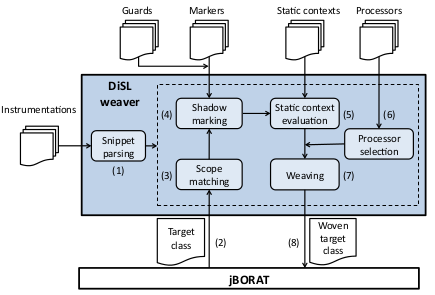
\includegraphics[scale=0.5]{images/Languages/DiSL_Weaver.png}\\
\caption{Overview of DiSL weaving process.\citep{marek_disl:_2012}}
\label{fig:DiSL_Weaver}
\end{figure}

\section{Examples}
\begin{lstlisting}[language=Java,caption=Aspect for calling context-aware profiling.,label=lst:DiSL_ExampleProfiler]
public class CallingContextBBAnalysis {
	@ThreadLocal
	static CCTNode currentNode;

	@SyntheticLocal
	static CCTNode callerNode;

	@Before(marker = BodyMarker.class, order = 1)
		static void onMethodEntry(MethodStaticContext msc) {
		if ((callerNode = currentNode) == null) {
			callerNode = CCTNode.getRoot();
		}
		currentNode = callerNode.profileCall(msc.thisMethodFullName());
	}

	@After(marker = BodyMarker.class)
	static void onMethodcompletion() {
		currentNode = callerNode;
	}

	@Before(marker = BasicBlockMarker.class, order = 0)
	static void onBasicBlock(BasicBlockStaticContext bbsc) {
		currentNode.profileBB(bbsc.getBBIndex());
	}
}
\end{lstlisting}
\begin{lstlisting}[language=Java,caption=Example for collecting run-time information.,label=lst:DiSL_ExampleSenseo]
public class Senseo {
	@ThreadLocal
	static CCTNode currentNode;
	
	@SyntheticLocal
	static CCTNode callerNode;	
	
	@Before(marker = BodyMarker.class, order = 1)
	static void onMethodEntry(MethodStaticContext msc, ArgumentProcessorContext proc) {
		if ((callerNode = currentNode) == null) {
			callerNode = CCTNode.getRoot();4
		}
			
		currentNode = callerNode.profileCall(msc.thisMethodFullName());
		proc.apply(ReferenceProcessor.class, ProcessorMode.METHOD_ARGS);
	}
	
	@After(marker = BodyMarker.class, order = 2)
	static void onMethodCompletion() {
		currentNode = callerNode;
	}
	
	@AfterReturning(marker = BodyMaker.class, order = 1, guard = MethodReturnsRef.class)
	static void onReturnRef(DynamicContext dc) {
		Object obj = dc.getStackValue(0, Object.class);
		currentNode.profileReturn(obj);
	}
	
	@AfterReturning(marker = ByteCodeMarker.class, order = 0, args = "new,newarray,anewarray,multianewarray")
	static void onAllocation() {
		currentNode.profileAllocation();
	}
	
	@Before(marker = BasicBlockMarker.class, order = 0) {
	static void onBasicBlock(BasicBlockStaticContext bbsc) {
		currentNode.profileBB(bbsc.getBBIndex());
	}
}

@ArgumentProcessor
public class RefferenceProcessor {
	static void objProc(Object obj, ArgumentContext ac) {
		Senseo.currentNode.profileArgument(ac.getPosition(), obj);
	}
}	
\end{lstlisting}


\section{Difficulties}
DiSL is a language completely different from those discussed until now. Despite this difference the framework is still able to provide useful functionality proving its value. Besides some minor difficulties, mostly caused by the lack of functionality, there are no big problems if this were to be created with the framework. All the tools that are used to aid in creating this language could also be used when working with the framework.

\chapter{Discussion}
\label{chap:Discussion}
As demonstrated by the languages presented and discussed in the previous chapters, the framework is general enough to be useful in a wide range of languages. The amount of work required to extend the framework depends on the complexity of the target language, and is mostly dominated by the effort required for the weaver. Thanks to the presence of 'helper' methods in the general Weaver class, the work that has to be put into the weaver is limited to putting everything together, and finding matches is already done for us.\\
\\
In general we experience that the concept of pointcuts and advice, as it is represented by the framework, provides a good basis to start from. The extensions that are required are very limited. The entire type system however, because it can not be provided by the framework may cause to be problematic. Though if handled well, it is possible to simply reuse the existing type system of the base language eliminating the cost of creating a complete new one.\\
\\
The poincutset which was meant as a way to simplify selecting multiple join point that could not be selected by wildcards proves to be very useful, though it still has room for improvement since the only supported operator is the logical or. As most other AOP languages support other operators as well, this may seem to be a very limited way to express a set of pointcuts. Upon closer inspection this is often not the case, since for most join points it makes no sense to require that it should happen together with another join point. If we look at the some examples of AspectJ, we note that the '\&' is used with the \textbf{within} keyword. This however is not a join point and is therefore part of the context in the framework.\\
\\
The extended framework and the base language only interact with a compiler that extracts the join points from the source code, and with the weaver that adds the advice in the right place. This is however not the only coupling between the base language and the framework, most components that are added to support AOP for the base language will carry some notion of the base language, being it implicitly. More coupling between the framework and the base language is the type system which is preferably the same.\\
\\
Finally we note that modifying the parser for the base language to extract the join points can be quite cumbersome. One way to minimize the required effort would be to use an existing aspect-oriented language and inject the modifications as advice. This way of working is however very limited and can only be done if there is a match between the join point model of the aspect-oriented language and the interesting points in the parser. If we would for instance use AspectJ, we are limited to the beginning and end of method executions and calls. If the parser is not sufficiently organized it is impossible to add the code at the right place and the entire approach can not be applied without modifications to the parser.

\chapter{Future Work}
\label{chap:FutureWork}
The languages discussed in this thesis have shown some limitations of the framework. The most important one is the lack of communication between advice. This could be solved by introducing global variables, which would be similar to arguments currently present for advice. The weaving step would have to be extended depending on the way the variables are woven with the base language source code.\\
\\
Many other AOP languages have an explicit notion of aspect, this is not the case in this framework but could be considered as a valuable addition. Before doing so, it is essential that some questions are answered. Will the aspect only be used to encapsulate variables, pointcuts and advice or will it be possible to use it like classes in an object-oriented language? If that is the case then we gain some valuable features, such as the reusability of pointcuts. However inheritance would also apply for advice, which means we need a way to select the right advice in case they are overridden. Another problem would be to choose between multiple subaspects, certainly since this choice may not be the same for the entire application, but can differ from join point to join point.\\
\\
Another problem with the current framework is the lack of choice between different ways of weaving. Though it is possible to weave the original files and the advice any way desired, it is the time of weaving that lacks freedom. The only real option is using the weaver as a pre-processor. This should be extended to provide more support for run-time weaving, since adding run-time checks isn't always feasible.\\
\\
Another important feature still missing is decent support for debugging, as this is completely left to the compiler of the target language. This however means that all errors are reported based on the woven code instead of the original source and aspect files. The easiest way to do this is to encapsulate the final compiler and intercept the errors. By keeping track of the woven locations we can resolve the errors back to the original locations. This approach can not only be done for 'fixing' the reported errors, but could also be used to handle other tools that work on the woven code.\\
\\
Currently the framework treats context and arguments in a different way, and the notion of a context is closer to a type, as they both define an interface with just an \textbf{isAssignable} method. We could ask ourselves in what way a context would be different from an argument, since in most cases a context variable will have a name and a value, just as an argument.\\
\\
Finally also the weaving process could be optimized to handle quick re-weaving. Currently the weaver starts from the original files every time the process is started. This requires a lot of time for large projects and a lot of woven code will be the same as the previous, since often only small changes are made at a time. Achieving this involves adding links between the aspect code and source code, which is also required to 'fix' the error messages mentioned earlier.

\chapter{Related Work}
\label{chap:RelatedWork}
Language Oriented Programming \citep{dmitriev_language_2004} is similar in that way that it provides freedom to the user to create his own DSL, just like the framework allows a user to specify his own aspect-oriented language. This is realized by implementing loosely coupled languages which can be combined as requested. Pluggable AOP \citep{kojarski_pluggable_2005} aims to specify aspect-oriented languages largely independent of the base language, which would allow combining multiple aspect-oriented languages together.  Though the approach is different as they don't use a framework but a description of the aspect-oriented language, both aim to get a loose coupling between the aspect-oriented language and the base language.\\
\\
Higher Order Attribute Grammars \citep{vogt_higher_1989} are a new kind of grammar that enables the structure tree to be extended as a result of attribute computations. This allows languages that can be more easily modified and enable extensions. This is shown in Aspects as Modular Language Extensions \citep{van_wyk_aspects_2003}, where they use a programming language that uses higher-order attribute to extend it with AOP. Where this thesis is about how we can add AOP to any type of language by having a general and modifiable framework, these papers are about how we can add AOP to modifiable languages. We might be able to use (parts of) this technique in the framework.\\
\\
XAspects \citep{shonle_xaspects:_2003} is a framework for aspect compilation that allows to combine multiple domain-specific aspect extensions. It does this by reducing all extensions to a single general-purpose aspect extension (AspectJ). This is an alternative to the type of framework presented in this thesis, but is not as general, since not all aspects can be reduced into AspectJ.\\
\\
In Towards An Aspect-Oriented Language Module: Aspects For Petri Nets \citep{molderez_towards_2012}, the concept of AOP is added to Petri Nets. Since this is clearly not a standard textual programming language such as Java, the entire idea is examined. It is shown that AOP is meaningful outside the current scope of its use, which supports the design of the framework in this paper.


\chapter{Conclusion}
\label{chap:Conclusion}
The provided functionality of the framework is still somewhat limited. Nevertheless it is able to achieve an abstraction of the core elements of aspect-oriented programming and has been successfully instantiated to prove its abilities, and its limitations. Despite the limitations of the current framework, it is often already possible to solve the problem in a different way. Yet adding new features and extensions will allow serving an even larger amount of languages and make the framework more user-friendly.

\bibliographystyle{plain}
\bibliography{references}

\end{document}